% \subsubsection{Challenges of Keyword-Based Location Disclosure}

% The rapid adoption of smart phones and tablets has led to innovative applications and services
% that exploit location information. Location information is increasingly used to
% drive advertising -- location-based targeting generates four times as much revenue per impression compared to ads 
% without location data\footnote{\url{http://bit.ly/vXWdsw}}. Even brick-and-mortar stores use location data, with retailers 
% using cell phones' WiFi signals to learn where customers spend time in their stores\footnote{\url{http://nyti.ms/15vLRva}}.

% There are many privacy concerns surrounding the use of this data.
% %Location information is more sensitive than other types of personally identifiable information (PII) not only because it can reveal private activities, but because knowledge of a person's physical presence creates the possibility of physical harm.
% For example, many applications access location information even when such information is not needed, and may share it 
% with multiple third parties, leading to privacy concerns~\cite{Enck:2010, WSJ:apple} and attracting 
% the attention of regulators~\cite{USC:location, jones2012us}.
% This work focuses on location information generated in real-time by users with mobile devices.

Many privacy concerns around location information are rooted in the mobile application ecosystem.
Most mobile services and applications are free and operate by collecting 
personal information (browsing activity, location, etc.) and monetizing this information 
through targeted ads~\cite{Leontiadis:2012}. 
% Because it affects their profits, companies that are a part of the mobile application ecosystem oppose any regulation that may restrict access to location data and claim that the ``cost'' of a privacy bill threatens the web's general economy and ultimately hurts customers. 
In fact, one may argue that users today exchange their data for services.
An ideal privacy solution therefore should provide adequate privacy protection to the user while simultaneously enabling service providers to collect and monetize data. 
Our objective is to lay the groundwork for a comprehensive and deployable solution to location privacy. 

In this section, I describe published work~\cite{Riederer:2013ila} that aims to reconcile the users' control over their location information with its commercial value.
This approach raises three challenges:
(1) The solution should be \emph{incrementally deployable}. 
It must easily integrate with current devices and practices while giving all parties an incentive to participate.
(2) The solution should be \emph{robust} against threats from its participants. 
Advertisers should not be able to access data without compensating users or access more than the users specify. 
Users should not be able to benefit from seeking unfair compensation.
(3) The solution should be \emph{easy to use}. 
The system should be easily understood by both users and advertisers.

Our solution is based on selective disclosure; users decide what location information they want to disclose.
At the heart of our solution is a \emph{keyword-based} method where keywords are associated with locations, and the decision to release locations is based on keywords. 
We observe that keywords are naturally associated with the elements that define this problem, but also offer a strong abstraction to handle location data.  
In order to drive the adoption of the solution, we propose providing economic compensation to the users for the location information they disclose. 
Application and web service providers bid to gain \emph{access} to users at these specific locations in real-time. 

\subsection{Overview}
Our requirements calls for a solution to share information about location monetized by ad-networks and 3rd party aggregators through \emph{selective disclosure}. For the user to retain control, our privacy solution should address \emph{how} the information is released, under \emph{which conditions} the information is released and to \emph{whom}, as seen in previous ones, e.g.~Koi~\cite{guha:koi}, 

% To meet our requirements, we create a solution based around \emph{selective disclosure}; users disclose location information that they are willing 
% to release.
% This information is monetized by ad-networks and third party aggregators by way of online ads. 
% The control remains with the user. 
% Any privacy solution based around selective disclosure 
% needs to
% address 
% \emph{how} the information is released, under \emph{which conditions} the information is released and to \emph{whom}.

To specify \emph{how} and \emph{under which conditions} location information is released, we choose to use keywords. 
While the information that is released is a latitude longitude pair (lat-long), the decision to disclose is based on associated keywords. 
Users who are comfortable disclosing location under certain circumstances~\cite{Kelley:2011} opt-in to reveal lat-long associated with keywords of their choices.
%
% In order to answer \emph{how} we release location information, we design our solution around keywords
% associated with locations; the decision to release is based on keywords associated with locations, and
% the information that is actually released is the location. %% IS IT THE LOCATION, OR THE KEYWORD?
An example would be a street that has many restaurants serving different cuisines, it would have keywords like ``restaurant, Thai, French, Indian'' associated each with the lat-long of each particular venue. 
The use of keywords brings important advantages: 
(i) Keywords let us deal with the problem of location privacy at a higher abstraction than coordinates or even location descriptors as in Koi~\cite{guha:koi}. 
(ii) Keywords are user friendly: instead of having to decide the sensitivity of every location, users decide on a much smaller set of keywords that they are comfortable releasing or not.
(iii) Today's ad-networks function primarily around keywords, thereby a solution around keywords can make it easier for ad-networks to adopt and use.
(iv) As there can be a finite set of keywords associated with any location, and the association of a keyword with a location typically remains for long periods of times, modifying keywords associated with a location is easy, making the solution scalable. 

Our solution compensates users \emph{economically} for information they release to aggregators and ad-networks. Economic incentives can nudge more users towards adoption, as concerns about privacy alone are rarely sufficient. Concrete incentives also sometimes reduce users' cognitive biases when it comes to perceiving their privacy~\cite{loewenstein2010misplaced}. Specifying to \emph{whom} the information is released is implicitly done by a market. 
%They also addresses the issue of to \emph{whom} the information will be released to -- parties that can pay. 
In principle, any parties that can pay for it is legitimate. In practice, this agreement should be facilitated by a trusted third party who vet the parties and send information about the user \emph{only} for locations she agreed on, upon payment. 

\begin{wrapfigure}{R}{0.5\textwidth}
% \begin{figure}[t]
  \begin{center}
    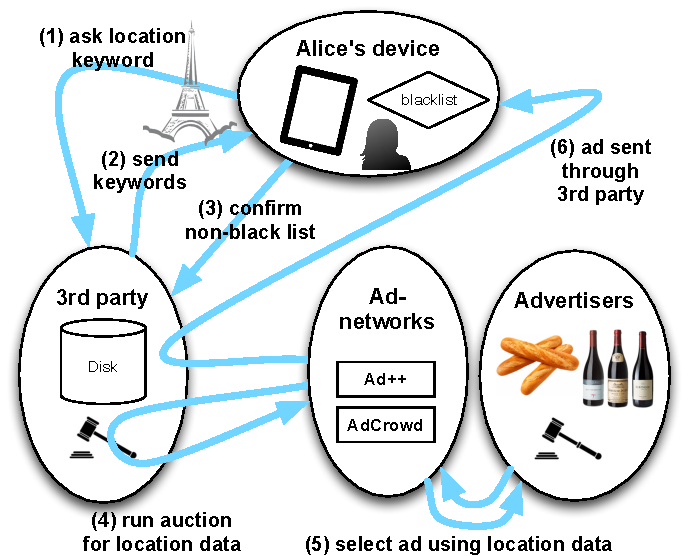
\includegraphics[width=0.9\linewidth]{fig/keyword/TLPOverview.pdf}
  \end{center}
  \caption{Solution overview}
  \label{fig:overview}
% \end{figure}
\end{wrapfigure}
The architecture consists of the following components: 
(i) a keyword server which maps physical locations to keywords
(ii) a location blacklist module which contains a list of sensitive keywords, 
communicates with the keyword server, and reveals non-sensitive locations
(iii) a blocking module in the network that blocks access to various parties, 
% (ii) a blacklist module that contains a list of sensitive keywords and maps these
% keywords to physical locations -- these are locations that will not be revealed, 
(iv) a market that puts up for sale information about locations visited by the user that are not in the blacklist, 
and (v) a module that grants \emph{access}
to the user for parties that pay, after purchasing access on the market.
With the exception of (ii), which can be a simple smartphone app, all modules are stored in the network; \emph{no} changes are required on the device.

A high-level diagram is shown in Fig.~\ref{fig:overview}. 
We describe the process with a simple example. 
Alice is willing to share certain locations and would like to hide her presence at other locations, a typical occurrence~\cite{Kelley:2011}. 
Alice wants to buy bread, shop for wine, and go to the Libertarian party headquarters. 
She would like to conceal her political leanings.
Alice would therefore put `Libertarian, Politics' as keywords in her \emph{blacklist module}. 
% We describe in Sec.~\ref{subsec:implementation} how the blacklist formation can be simplified through nested menus and re-ordering. 
% This blacklist will be stored on a server at a third party location. 
We assume the third party is trusted and leave lowering this requirement to future work.


\subsection{Deployment and User Study}
An implementation consists of the five components:
a keyword server, a location blacklist module, a network blocking module, an information market, and an access module.

% (i) a keyword server which maps keywords to physical locations
Our \textbf{keyword server} used Yelp's API.  % TODO: cite Yelp
Each time a device uploaded a lat-long to the server, we queried Yelp to find the categories of each location within 50 meters, using these categories as the location's keywords.
The \textbf{location blacklist} module was written as an Android application. 
The app was designed to give users a way to edit a blacklist and monitor which locations (and corresponding keywords) were being recorded. 
We used Yelp's 885 categories as our keywords during the study, meaning users had a large number of potential keywords to blacklist.
To make adding keywords to the blacklist manageable, all possible keywords were placed in a nested menu by category. 
We placed categories previously defined to be sensitive~\cite{bing} near the top of this list, and alphabetized all potentially less sensitive categories.
The blacklist was stored locally on the phone. 
\emph{At no point did the authors have access to a study participant's blacklist.}
Each half hour, the app would passively check the keywords in the current location and upload the location and keywords to the server only if no keywords were on the blacklist.
For the purposes of our small scale user study, we did not create a \textbf{blocking module} or connect the system to any ad exchanges.

\begin{wrapfigure}{R}{0.5\textwidth}
% \begin{figure*}[!htb]
% \minipage{0.32\textwidth}
%   \centering
%   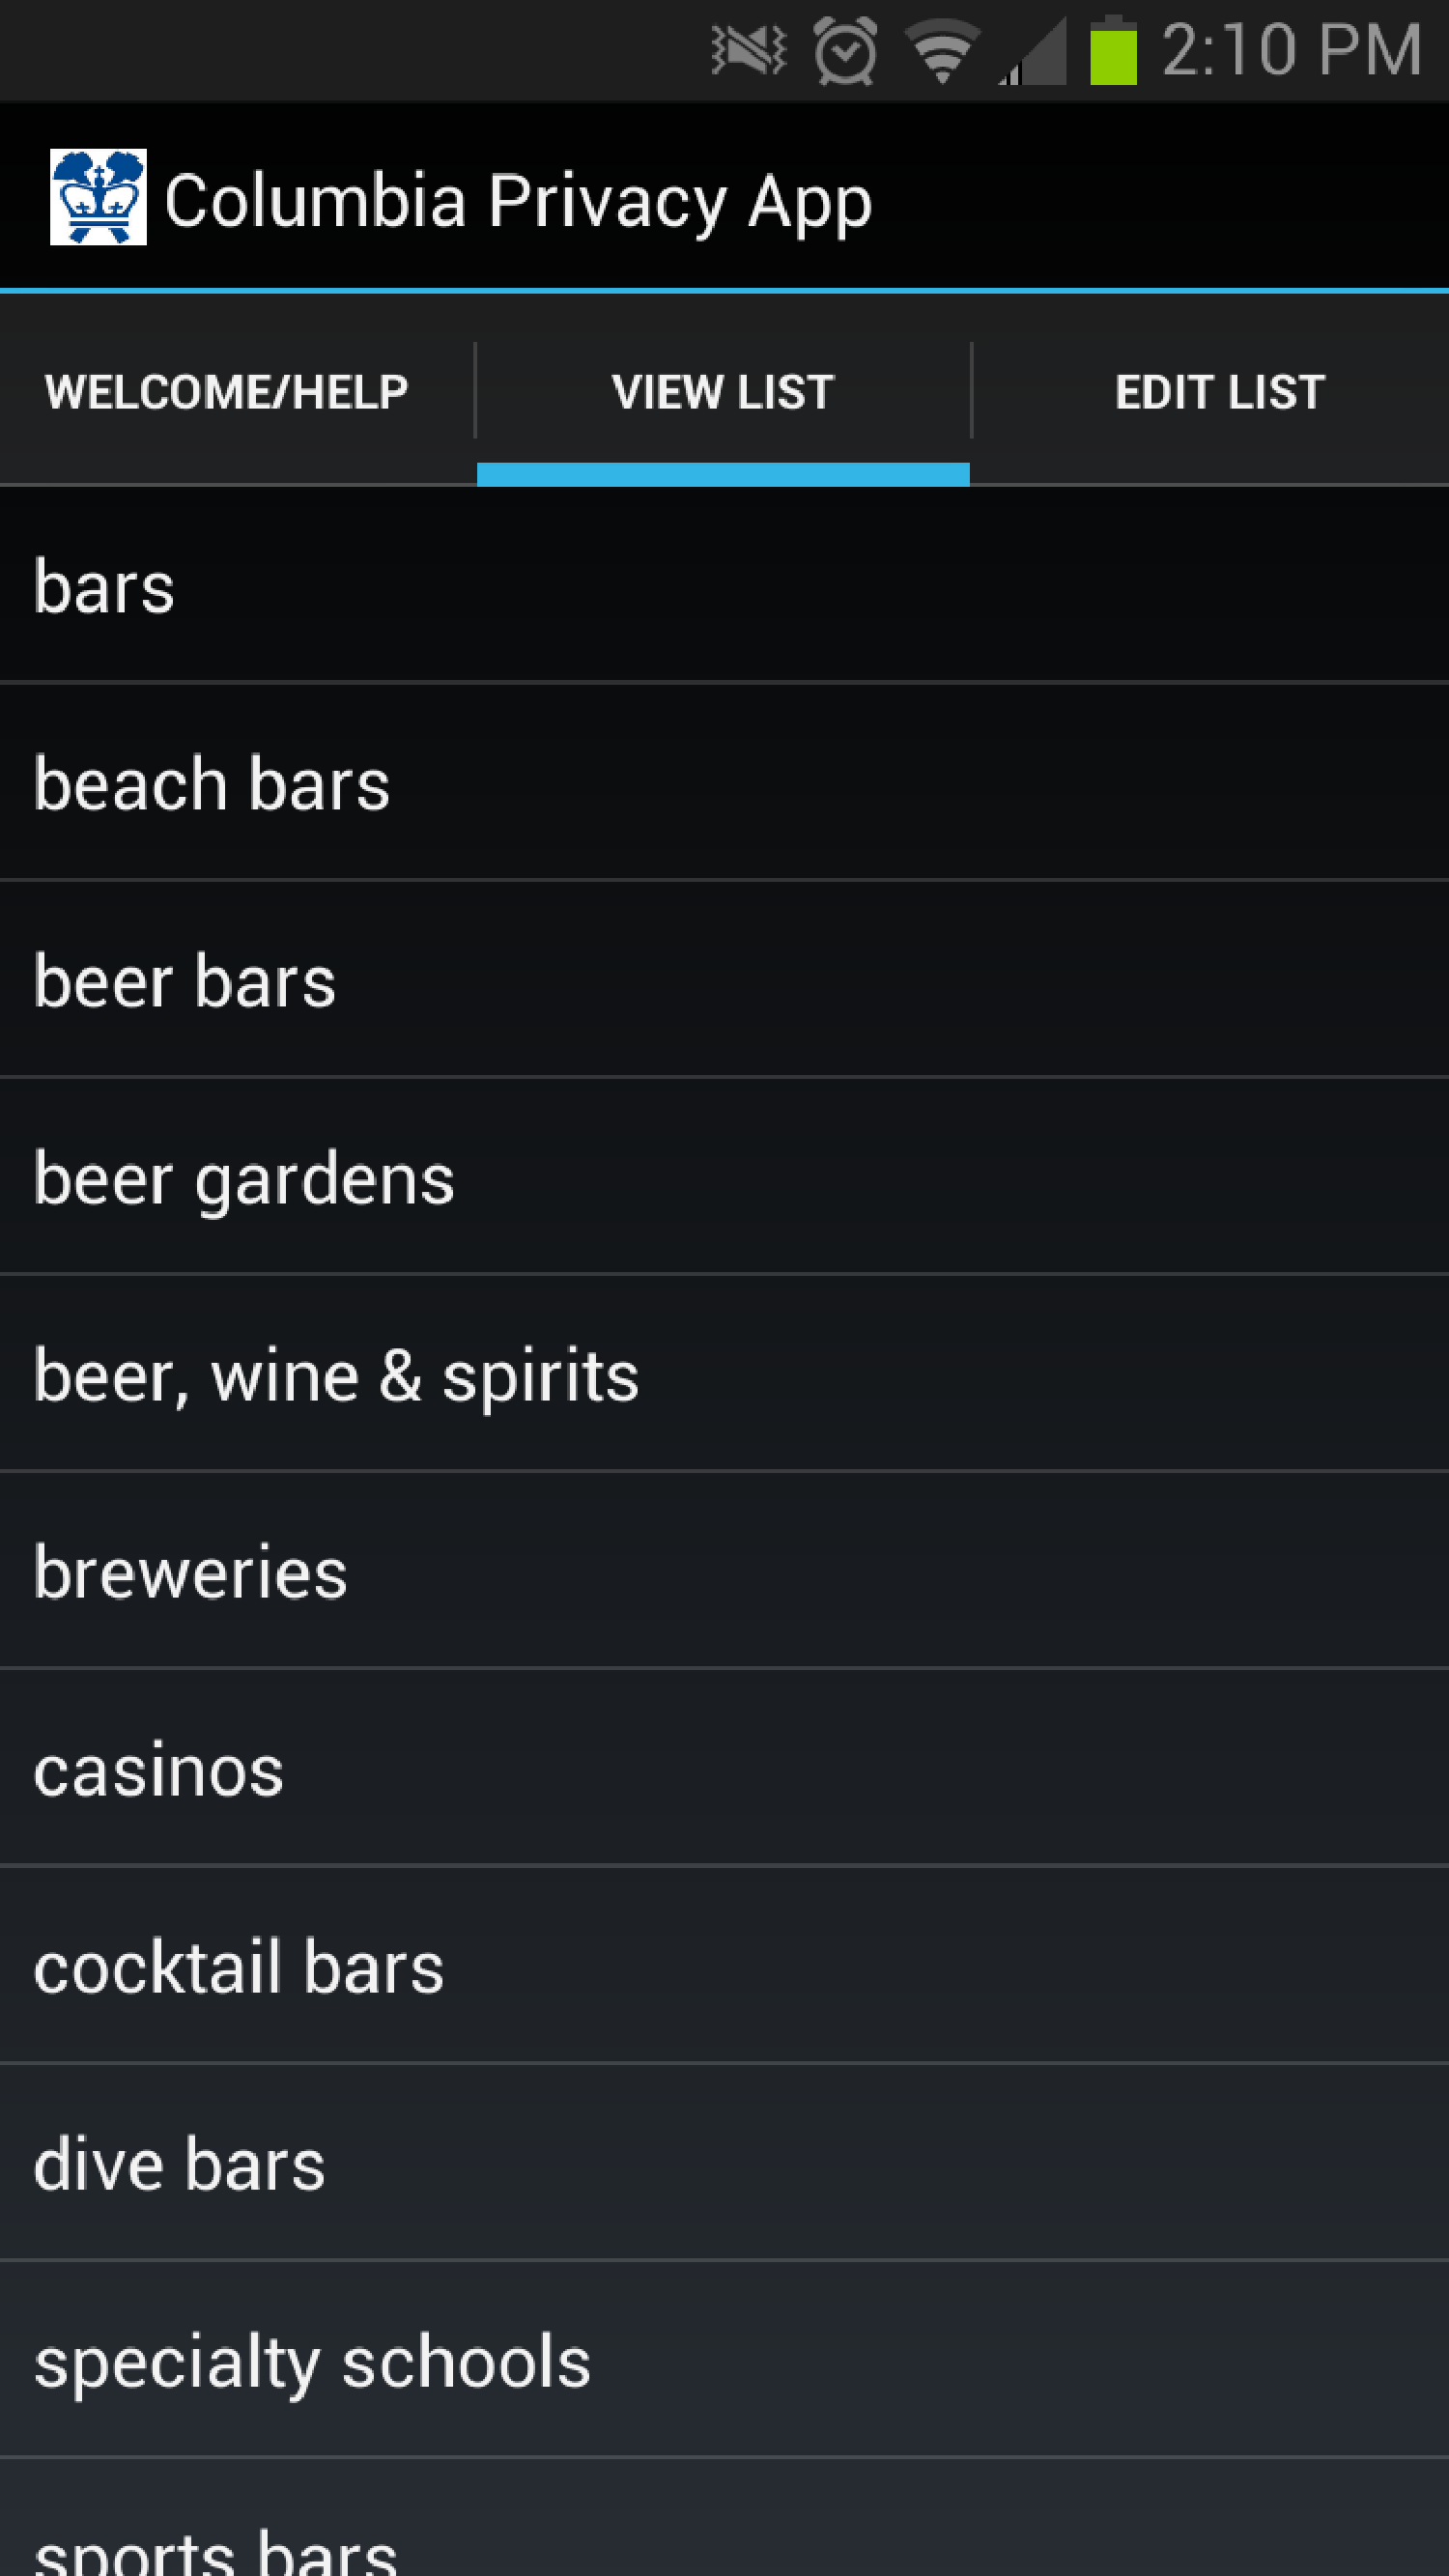
\includegraphics[width=0.75\linewidth]{./fig/screenshot_blacklist.pdf}
%   \caption{Blacklist}\label{fig:awesome_image1}
% \endminipage\hfill
\minipage{0.25\textwidth}
  \centering
  \includegraphics[width=0.75\linewidth]{fig/keyword/screenshot_addlist.pdf}
%  \caption{Adding screen}\label{fig:awesome_image2}
\endminipage\hfill
\minipage{0.25\textwidth}
  \centering
  \includegraphics[width=0.75\linewidth]{fig/keyword/screenshot_map.pdf}
%  \caption{Map}\label{fig:awesome_image3}
\endminipage
\caption{User Interface: (left) managing keywords black list, (right) visualizing locations released.}
\end{wrapfigure}

Instead of implementing a \textbf{market} or \textbf{access module}, we simulated the incentives and costs a user might experience while using our system. 
In our deployment, all participants received \$10 for participating and were entered into a lottery.
Each user was instructed that releasing more `valuable' information would give them a higher chance of the lottery.
We did not disclose the exact method of valuing information, mimicking the opaque way in which information would be priced in a real implementation of the system. 
The intention was that this would incentivize users to release more information.
To protect users' safety, users could contact us at any point if they were concerned about an unintentional location release. 
Additionally, any time a data point was recorded, we delayed making it public by 24 hours. 
Users could see their data points in real-time via a password-secured link.

We deployed our implementation with six users for two weeks. 
Users were geographically diverse, located in multiple cities throughout the United States.
Study participants were recruited through advertising on social networks and were primarily adults in their mid-twenties.

After the study, we asked users to complete a survey. 
Our study was too small to make general conclusions, but we present results here to inform future work. 
Users easily understood both the keyword system and the interface. 
Users were divided on how well they felt the system secured their privacy, with some users concerned that our mapping of keywords to locations was not precise enough. 
Our users expressed a range of privacy sensitivities. 
Some did not use the blacklist and others used the blacklist to hide sites they associated with social stigma or that they thought would send negative signals to employers, insurers, or the police.

% Maybe attacks on privacy


% \section{Introduction}
\label{sec:intro}

% Broad topic
% Specifics of topic and importance
% Previous gaps we're trying to address
% Core research challenge
% Roadmap

%VE: too much intro stuff. Just need one para!
% Overview
%When it comes to privacy, one of today's most widely open problems is posed by location information. Knowing \emph{where} a user is \emph{at any time} is remarkably sensitive but also extremely informative and valuable. Mobile devices such as smartphones and tablets, which represent a growing fraction of users' browsing time, make it increasinlgy easy to capture, store and monetize users' real-time locations. 

% Importance: value of LI
% Narrow LI down to realtime mobile devices
The rapid adoption of smart phones and tablets has led to innovative applications and services
that exploit location information. Location information is increasingly used to
drive advertising -- location-based targeting generates four times as much revenue per impression compared to ads 
without location data\footnote{\url{http://bit.ly/vXWdsw}}. Even brick-and-mortar stores use location data, with retailers 
using cell phones' WiFi signals to learn where customers spend time in their stores\footnote{\url{http://nyti.ms/15vLRva}}.

There are many privacy concerns surrounding the use of this data.
%Location information is more sensitive than other types of personally identifiable information (PII) not only because it can reveal private activities, but because knowledge of a person's physical presence creates the possibility of physical harm.
For example, many applications access location information even when such information is not needed, and may share it 
with multiple third parties, leading to privacy concerns~\cite{Enck:2010, WSJ:apple} and attracting 
the attention of regulators~\cite{USC:location, jones2012us}.
This work focuses on location information generated in real-time by users with mobile devices.
%location information was the focus of a recent, major United States Supreme Court case~\cite{jones2012us}.
%Users also appear to desire access to location-based information, with 74\% of smartphone owners reportedly using their device to obtain real-time location-based information.

%new revenue streams for platform providers, application developers
%as well as traditional web 

%Knowing this information is very valuable, as location-based targeting can get four times as much revenue per impression compared to ads without location data~\cite{Loc:ad}.
%Even brick-and-mortar stores are interested in location data, with retailers using cell phones' WiFi signals to learn about how customers travel through stores~\cite{NYT:storeLoc}.
%Users also appear to desire access to location-based information, with 74\% of smartphone owners reportedly using their device to obtain real-time location-based information.
% TODO: CITE PEW
% Importance: privacy issues around LI
%At the same time, there are many privacy concerns surrounding this type of data.
%Location information is more sensitive than other types of personally identifiable information (PII) not only because it can reveal private activities, but because knowledge of a person's physical presence creates the possibility of physical harm.
%Concerns about location privacy have attracted the attention of regulators~\cite{USC:location, Cal:Location} and location information was the focus of a recent, major United States Supreme Court case~\cite{jones2012us}.
%Many web services and applications access location information even when such information is not needed, and may share it with multiple third parties, raising serious privacy concerns~\cite{Enck:2010, WSJ:apple}. 

% Background: Brief description of online advertising
Many privacy concerns around location information are rooted in the mobile application ecosystem.
Most mobile services and applications are free and operate by collecting 
personal information (browsing activity, location, etc.) and monetizing this information 
through targeted ads~\cite{Leontiadis:2012}. 
% This is why, when privacy advocates request stricter rules to be enforced on information collection, they typically are opposed by companies providing these services. 
Because it affects their profits, companies that are a part of the mobile application ecosystem oppose any regulation that may restrict access to location data and claim that the ``cost'' of a privacy bill threatens the web's general economy and ultimately hurts customers. 
In fact, one may argue that users today exchange their data for services.
%Privacy advocates ask for stricter regulation on information collection, while service and application providers argue that it would jeopardize the thriving economy of the mobile web. 
An ideal privacy solution therefore should provide adequate privacy protection to the user while simultaneously
enabling service providers to collect and monetize data. 
Our objective is to lay the groundwork for a comprehensive and deployable solution to location privacy. 
%Indeed, mobile privacy solutions often fail to gain traction as users judge it profitable to disclose some location information in exchange for compensation, which is found in the form of a free convenient service. A comprehensive privacy solution, in contrast, should ideally allow users to opt-in for some information disclosure when they find it profitable. 


% What is the specific problem to address?
% The value, sensitivity, and ease of collection of location information has led to a potentially unsustainable situation. As the technologies to capture, store, and monetize location information continues to improve, public opinion may rapidly shift, leading to legislation that bans location collection and chokes off this promising new economy. We hope to find a balanced middle ground between the producers and consumers of location information before such a situation arises.
% Not surprisingly, this has opened a heated debate: 

% Main contribution
%The objective of this paper is to lay the groundwork for a comprehensive and deployable solution to this location privacy issue. In contrast to previous works, we aim at reconciling the control users exert over their data with its commercial value.
%This raises three main challenges:

%The solution should be \emph{incrementally deployable}: it must easily integrate with current devices and practices while giving all parties an incentive to participate.

%The solution should be \emph{robust} against threats to its participants. Advertisers wishing to access data without compensating users, or access more than the users specify, should be stopped. Users privacy should be protected, but they should also not be able to receive unfair compensation.

%The solution should be \emph{easy to use}: users and advertisers have to express their needs in intuitive terms.

In contrast to previous work, we aim to reconcile the users' control over their location information with its commercial value.
This approach raises three challenges:
(1) The solution should be \emph{incrementally deployable}. It must easily integrate with current devices and practices while giving all parties an incentive to participate.
(2) The solution should be \emph{robust} against threats from its participants. Advertisers should not be able to access data without compensating users or access more than the users specify. Users should not be able to benefit from seeking unfair compensation.
(3) The solution should be \emph{easy to use}. The system should be easily understood by both users and advertisers.

Our solution is based on selective disclosure; users decide what location information they want to disclose.
At the heart of our solution is a \emph{keyword-based} method where keywords are associated with locations, 
and the decision to release locations is based on keywords. 
We observe that keywords are naturally associated with the elements that define this problem, but also offer a strong 
abstraction to handle location data.  In order to drive the adoption of the solution,
we propose providing economic compensation to the users for the location information they disclose. 
Application and web service providers bid to gain \emph{access} to users at these specific locations in real-time. 

%As we show later, very few works to date attempt at managing the inherent value-risk tradeoff of personal data. Arguably, no system satisfies even two of the above conditions. 
%We propose a novel direction through a \emph{keyword-based} privacy solution grounded on a data market. We observe that keywords are naturally associated with the elements that define this problem, but also offer a strong abstraction to manipulate location data. In a nutshell, users decide what locations to release for commercial use and are compensated in return. Application and web service providers pay to gain \emph{access} to users at these specific locations, in real time. 
Our main contributions are:
% \begin{itemize}
(1) The design of a keyword-based system that integrates well into today's location collection and monetization. Our solution requires no change on users' devices, a minimum level of indirection, and addresses goals like usability, deployability and
scaling (Sec.~\ref{sec:overview}).
(2) A test of our solution's usability and relevance with a small scale trial on real users. While this experiment is too small to form statistically significant conclusions, it allowed us to test the feasibility of our design (Sec.~\ref{sec:user-study}).
(3) An analysis of how such a system can offer different levels of protection against various threats, including freeriding, 
inference attacks using auxiliary information, and user misconduct (Sec.~\ref{sec:security}).
% \item An evaluation of a deployment within the economy of mobile advertising. We use data gathered from cell phone users, geo-located services, ad-networks, and a simple revenue model. We found multiple privacy-value tradeoff that benefit users and advertisers. We find that if information is removed about most privacy sensitive locations, revenue drops by around 20\% (Sec.~\ref{sec:economic-analysis})
% \end{itemize}

%These results suggests the feasibility and promise of a solution centered on keywords. They more generally motivate to revisit how to reconcile user's location privacy with the economic interest of the mobile web. The deployment of this system poses multiple questions for each of these challenges in the long term, that we briefly discuss separately. 

% % Challenges / Requirements
% In order to realize and analyze transactional location privacy, several challenges have to be met.
% The system has several important requirements:
% \begin{itemize}
% \item The system must give control to users over what information is released to advertisers.
% \item The system needs to be user-friendly, giving both users and advertisers an intuitive way of thinking about labeling locations of different sensitivities.
% \item The system must operate in real time and be architected in a way that preserves the users's privacy.
% \item The system must not be vulnerable to attacks by users seeking to get unfair compensation or by advertisers seeking to infer more information than a user wishes to reveal.
% \item Typical use of the system should not greatly reduce an advertiser's potential revenue.
% \end{itemize}
% We hope to meet all of these requirements in the design of our system.
% % Or make paragraphs-- one detailing system needs, one emphasizing user issues, one talking about economics.
% 
% % Main results
% 
% 
% % Paper Roadmap
% The paper is laid out in the following manner:
% Related work is discussed in Sec.~\ref{sec:relwork}.
% The system architecture is described in Sec.~\ref{sec:overview}. 
% The security of the system is described in Sec.~\ref{sec:security}.
% The economic implications of the system is described in Sec.~\ref{sec:economic-analysis}.
% A description of our user study is included in Sec.~\ref{sec:user-study}.
% Finally, we conclude in Sec.~\ref{sec:conclusion}.

% \section{Overview}
\label{sec:overview}
%In this section, we provide our assumptions, a description of the design, a simple example to explain how our solution works, and enumerate the advantages of the system.
This section presents the motivation, design and advantages of a location disclosure system based on keywords. 

\subsection{A keyword-based solution}
\label{subsec:key}

% Location information\footnote{we focus on location information that can be collected via mobile devices} 
% has the following properties: 
% (i) it is considered more sensitive than other types of personal information and more valuable, 
% (ii) its utility is transient in many cases;
% for targeting reasons knowing real-time location is often more useful than knowing location later, 
% (iii) it is predictable; mobility patterns have been shown to be periodic~\cite{salva}.  

Our requirements calls for a solution to share information about location monetized by ad-networks and 3rd party aggregators through \emph{selective disclosure}. For the user to retain control, our privacy solution should address \emph{how} the information is released, under \emph{which conditions} the information is released and to \emph{whom}, as seen in previous ones, e.g.~Koi~\cite{guha:koi}, 

% To meet our requirements, we create a solution based around \emph{selective disclosure}; users disclose location information that they are willing 
% to release.
% This information is monetized by ad-networks and third party aggregators by way of online ads. 
% The control remains with the user. 
% Any privacy solution based around selective disclosure 
% needs to
% address 
% \emph{how} the information is released, under \emph{which conditions} the information is released and to \emph{whom}.

To specify \emph{how} and \emph{under which conditions} location information is released, we choose to use keywords. 
While the information that is released is a latitude longitude pair (lat-long), the decision to disclose is based on associated keywords. 
Users who are comfortable disclosing location under certain circumstances~\cite{Kelley:2011} opt-in to reveal lat-long associated with keywords of their choices.
%
% In order to answer \emph{how} we release location information, we design our solution around keywords
% associated with locations; the decision to release is based on keywords associated with locations, and
% the information that is actually released is the location. %% IS IT THE LOCATION, OR THE KEYWORD?
An example would be a street that has many restaurants serving different cuisines, it would have keywords like ``restaurant, Thai, French, Indian'' associated each with the lat-long of each particular venue. 
The use of keywords brings important advantages: 
(i) Keywords let us deal with the problem of location privacy at a higher abstraction than coordinates or even location descriptors as in Koi~\cite{guha:koi}. 
(ii) Keywords are user friendly: instead of having to decide the sensitivity of every location, users decide on a much smaller set of keywords that they are comfortable releasing or not.
(iii) Today's ad-networks function primarily around keywords, thereby a solution around keywords can make it easier for ad-networks to adopt and use.
(iv) As there can be a finite set of keywords associated with any location, and the association of a keyword with a location typically remains for long periods of times, modifying keywords associated with a location is easy, making the solution scalable. 

Our solution compensates users \emph{economically} for information they release to aggregators and ad-networks. Economic incentives can nudge more users towards adoption, as concerns about privacy alone are rarely sufficient. Concrete incentives also sometimes reduce users' cognitive biases when it comes to perceiving their privacy~\cite{loewenstein2010misplaced}. Specifying to \emph{whom} the information is released is implicitly done by a market. 
%They also addresses the issue of to \emph{whom} the information will be released to -- parties that can pay. 
In principle, any parties that can pay for it is legitimate. In practice, this agreement should be facilitated by a trusted third party who vet the parties and send information about the user \emph{only} for locations she agreed on, upon payment. 

%At a high-level the core of our solution is based on involving the user in the economic value-chain
%that exists today around location information. The players that constitute this ecosystem include
%web content providers and application developers on one side whose respective offerings are often `free'. 
%On the other side are users who come attracted to the free offerings. 
%In addition, data aggregators
%and ad-networks who work with content providers and developers. 
%They collect information (including location) about users of applications and 
%monetize information by way of online ads. These ad-networks are in turn paid by advertisers. 
%A fraction of the revenue generated is passed on to
%application developers and content providers. 



% \textbf{Assumptions}
% As our solution is centered around economic transactions around location information, our architecture is designed for an honest-but-curious adversary. 
The design we next describe is meant to operate under the following set of \textbf{assumptions}. 
Given the amount of press on privacy related issues, we believe that the PR backlash in the case of a serious privacy violation will make such violations undesirable. As a consequence, we provision against an \emph{honest-but-curious} advertiser. It means the adversary complies with the system but it can exploit the information that is gathered for its own interest. We provide safeguards against inference and linkage attacks. We also assume that the mobile OS used complies with user's privacy, hence not sharing location information with any application once the user stated that request. 
Note that the architecture presented next is oblivious to a background service model (passive, potentially continuous tracking) or a check-in model. 

% Before describing the design, we first describe our \textbf{assumptions}.
% We consider our adversary to be an honest-but-curious advertiser. 
% This means our adversary participates in the system honestly but may try to exploit the information that is gathered.
% Hence our adversary is \emph{not} malicious. Applications leaking information to aggregators as well as aggregators involved
% in resale of data\footnote{like BlueKai~\url{http://www.bluekai.com/}} are not necessarily malicious, but honest but curious and economically motivated. 
% With this in mind, we provide safeguards against inference and linkage attacks.

% We provide safeguards against inference and linkage attacks. We do ensure that even if a link is established between a specific user and 
% a set of locations, no entity can gain economically with this information.

% We assume that once an entity enters into an agreement with the user, it is generally compliant. 
% We assume that location information can be tracked and gathered continuously, as this is the worst case. 
% In general this is not feasible as energy concerns around GPS usage will forbid this~\cite{energy:loc}. 


\subsection{Design and Example}
\label{subsec:design}

\begin{figure}[t]
	\begin{center}
		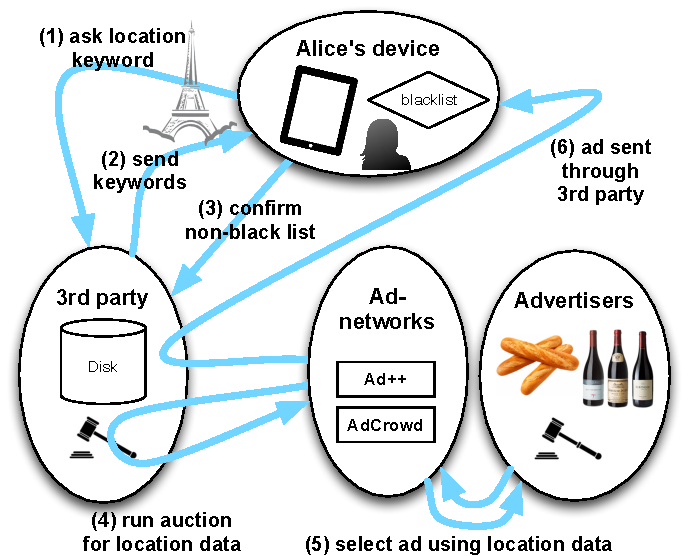
\includegraphics[width=0.9\linewidth]{fig/keyword/TLPOverview.pdf}
	\end{center}
	\caption{Solution overview}
	\label{fig:overview}
\end{figure}
The architecture consists of the following components: 
(i) a keyword server which maps physical locations to keywords
(ii) a location blacklist module which contains a list of sensitive keywords, 
communicates with the keyword server, and reveals non-sensitive locations
(iii) a blocking module in the network that blocks access to various parties, 
% (ii) a blacklist module that contains a list of sensitive keywords and maps these
% keywords to physical locations -- these are locations that will not be revealed, 
(iv) a market that puts up for sale information about locations visited by the user that are not in the blacklist, 
and (v) a module that grants \emph{access}
to the user for parties that pay, after purchasing access on the market.
With the exception of (ii), which can be a simple smartphone app, all modules are stored in the network; \emph{no} changes are required on the device.

A high-level diagram is shown in Fig.~\ref{fig:overview}. 
We describe the process with a simple example. 
Alice is willing to share certain locations and would like to hide her presence at other locations, a typical occurrence~\cite{Kelley:2011}. 
Alice wants to buy bread, shop for wine, and go to the Libertarian party headquarters. 
She would like to conceal her political leanings.
Alice would therefore put `Libertarian, Politics' as keywords in her \emph{blacklist module}. 
We describe in Sec.~\ref{subsec:implementation} how the blacklist formation can be simplified through nested menus and re-ordering. 
% This blacklist will be stored on a server at a third party location. 
We assume the third party is trusted and leave lowering this requirement to future work.

As Alice arrives at the bakery, her network activity goes through the \emph{blocking module} that runs a mix-network to conceal her real network address, and provides privacy protection like dropping cookies to third parties, overwriting \texttt{referer} headers etc.~\cite{Krishnamurthy:2007io} (see Sec.~\ref{subsec:implementation} for more on implementation).
At every location, Alice's device contacts the \emph{keyword server} which translates locations to keywords.
A check is then made against the blacklist to verify if Alice is comfortable releasing this information. 
If a location has multiple keywords and \emph{any} of them are on the blacklist, it is considered private.
% In order to perform this check, Alice's pwe need to translate the keywords to locations, described in Sec.~\ref{subsec:keywordmap}. 
Once a location passes the check, it is put on the \emph{market} for sale with a unique user-id and the keywords. 
This user-id is generated independently and can be periodically changed. 
The information then is ($UID_{Alice}$, (lat$_1$, long$_1$), Bakery). 
As she arrives at the wine shop, the information on the market will be ($UID_{Alice}$, (lat$_2$, long$_2$), Wine Shop), as the wine shop also passes the blacklist test. 
Ad-networks can pay to \emph{access} Alice based on these two locations released. 
The payment will be credited to Alice, with a small fraction taken by the third party. 
The third party then fixes a network address to reach Alice at the wine shop and conveys it to the ad-networks. 
Alice can receive a targeted ad (via an app or via SMS) for a particular wine.

As soon as Alice moves out of the wine shop, her network address changes and her location again is not known
to anyone but the trusted third party. 
When she is close to the Libertarian party headquarters, the check against the blacklist
returns a positive result, and this location is not revealed to anyone. 

% \subsection{Mapping Locations to Keywords}
% \label{subsec:keywordmap}
% Using a mapping of locations to keywords has a variety of challenges and advantages, which we now discuss.
% Locations may be defined in two ways which are both compatible with our system. It may denote a point of interest where users ``check in" (as in services like Foursquare) or alternatively it may represent a certain geographical area (defined using lat-longs or the coverage of a given cell tower).

% Creating a mapping of locations to keywords is not necessarily easy \emph{per se}, but one can reuse online services already providing such a mapping, such as Yelp, Google Places, and Foursquare.
% % This mapping can be obtained by gathering information from existing sites like Yelp, Google Places, or Foursquare.
% A ``folksonomy" approach could also be used where users augment the map over time, and even receive incentive. In this case, to encourage tagging of privacy-sensitive locations, the system can allow anonymous tagging. 
% Usability is also a challenge, and care must be taken to keep the number of keywords manageable and design the blacklist's user interface to be easy to use (see our UI in Sec.~\ref{subsec:implementation}).
% The keywords in the mapping will eventually be used by the user to specify a blacklist.
% Thus, 
% Yelp's hierarchical list of categories contains 885 entries, a reasonable number if handled properly in the UI.
% To specify a blacklist, a user need not look through every potential keyword. 
% Some ideas for the blacklist UI would be to group keywords into categories, where users can quickly decide if whole categories are sensitive or not, or can find specific words within a category that they think may be sensitive.
% % Rather, keywords can be grouped into categories, where users can quickly decide if whole categories are sensitive or not, or can find specific words within a category that they think may be sensitive.
% Additionally, categories that are more likely to be sensitive can be made more prominent in any blacklist creation software, by placing it at the beginning of a list, highlighting, etc. 


% \subsection{Design Specifics}
% \subsubsection{Blocking module}
% \label{sec:blocking}
% The purpose of this module is to block connections to prevent information leakage.
% Many mobile applications as well as web services rely on cookies to track the user,
% as well as send information to ad-networks and aggregators. 
% The connections to ad-networks and aggregators (AdMob, Flurry Analytics etc.) can be blocked by a proxy in the middle and by spoofing the MAC address. 
% All necessary proxies already exist: Privoxy comes with advanced filtering capabilities and handles rewrites of the HTTP headers like the `referrer' header to prevent leakages of any form, and mitmproxy can handle SSL\footnote{\url{www.privoxy.org}, \url{www.mitmproxy.org}}. 
% In addition, as the system works with opt-in users, we can have the users upload their SSH certificates to enable the module in the middle to masquerade as the user. 
% From an application's perspective, no logic is broken. 
% Even for location based services like Foursquare or maps, an unintentional checkin or a search at a private location can be prevented by checking against the blacklist -- an added benefit.  

% The proxy is part of a network of proxies that act as a mix network -- the real network address of the
%  mobile device will never be revealed to anyone. 

 %It is possible for manufacturers of mobile devices themselves
%to get information directly from the mobile device -- indeed Android seems to use SUPL to 

% \subsubsection{Blacklist module}
% \label{sec:blacklist}
% The objective of this module is to obtain the keywords for a user's current location, check the keywords against a blacklist, and then release the location if no keywords are blacklisted.
% The first step requires a mapping of locations to keywords.
% This mapping can be obtained by gathering information from Yelp, Google Places, or Foursquare.
% Additionally, a ``folksonomy" approach could be taken where users tag locations, building up a map over time.
% % Mention concern from paper: in folksonomy, sensitive places never covered?
% % In this case, users could again receive some incentive from 
% For simplicity and efficiency, the mapping of locations to keywords is on a central server.
% A user's blacklist is stored on her device, keeping this sensitive information away from a central point of attack.
% Encrypted queries from the device to the server in the form of lat-long coordinates will return keywords for that location.
% If no keywords exist for that location, a non-location-specific ad should be shown.
% The user's device can do a simple set intersection between the blacklist and the current location keywords and contact the ad-server accordingly.
% An open question is if zero-knowledge proofs can be used to notify a user of a location's keywords without the central server learning the user's location, thereby reducing the trust needed in the third party.

% A point of concern here is usability. 
% The number of possible keywords is probably on the order of 1000.
% To specify a blacklist, a user need not look through every potential keyword. 
% Rather, keywords can be grouped into categories, where users can quickly decide if whole categories are sensitive or not, or can find specific words within a category that they think may be sensitive.
% Additionally, categories that are more likely to be sensitive can be made more prominent in any blacklist creation software, by placing it at the beginning of a list, highlighting, etc.


\subsection{Summary of Advantages}
Now that we've described the system, we discuss the benefits of the system for various parties.
% There are benefits in the system for various parties.

\textbf{Users} obtain monetary payment for their data and privacy through choice.
The architecture operates in the network and hence, users do not need to make changes to their devices.
If information is leaked or shared between colluding ad-networks, these parties would have to gain access to the user to monetize this information -- and unless these parties have paid, they are prevented from gaining access to the user.
Hence, we protect against adversaries aiming to extract economic gain. 
We deal with adversaries who try to infer the identity of users or blacklisted keywords in Sec.~\ref{sec:security}.

The keyword system also benefits the user.
If a user is visiting a place they are unfamiliar with, they may not be accustomed to what areas are privacy sensitive.
Because keyword mappings work in any location, a user's privacy is protected even in unfamiliar areas.
Additionally, a user may simply not realize the privacy sensitive nature of a location they are in.
Because all traffic is directed through our system, if a user starts using a location-based service at a location they don't realize is privacy sensitive, our system can catch it and warn the user before they complete the action.

\textbf{Ad-networks and aggregators} can obtain non obfuscated data in a legal way, minimizing data breaches. As the data is `bought', the ad-networks can micro-target. 
Ad-networks and advertisers can easily make sense of the location data, as keywords are already used for context in current online advertising systems.
Rather than having advertisers need to bid specifically for each location, ad-networks can simply run auctions for ad impressions in locations associated with specific keywords. 

\textbf{Application developers} do not need to alter their code as we operate directly in the network. Applications serve as a conduit to show ads to the users, much as they do today. 



\textbf{Finally, mapping locations to keywords helps our system evaluation}.
Ad-networks constantly run many auctions of impressions to a customer searching for a specific term. Cost-per-click (CPC) data from ad-networks hence reflects the overall advertising demand on this topic. We show how CPC data may be collected and used to understand the economic value of locations.


% \subsection{Data-Driven Approach}
% \label{subsec:data}

% \begin{table*}
% \begin{center}
% \begin{tabular}{|r||c|c|c|c|}
%   \hline
%   % Percent Data Trained On & Foursquare & City A \\
%   Data set & Number Users & Number Checkins & Number Locations & Collection duration \\
%   \hline \hline
%   Foursquare & 40,578 & 1,377,181 & 460,663 & March-August 2011 \\
%   % CDR 		 & $\sim$ 2 mil & $\sim$ 800 mil & $\sim$ 7000 & 3 months, 2009-2010 \\
%   \hline
% \end{tabular}
% \end{center}
% \vspace{-3mm}
% % \caption{Data}
% \label{fig:freqtable}
% \end{table*}

% DO WE NEED ANOTHER SENTENCE HERE??
% To evaluate potential attacks, we used several large data sets. 
% % To evaluate potential attacks as well as investigate economic properties of our solution, we used several large data sets. 
% We gathered mobility patterns of a populations and geo-data to associate a location with a particular keyword.
% % , and (iii) estimates of the commercial value of advertising targeted at each keyword.
% To the best of our knowledge, no prior work ever combined them.
% % (??)
% % Meeting our objective requires to combine (i) representative mobility pattern of a large population, (ii) geo-data to associate a location with a particular commerce or terms, and (iii) estimation of the commercial value of advertising at this place. To the best of our knowledge, no prior work ever combined them.
% These data sets included:
% We used several large data sets to evaluate our model: %billions of anonymized call description records (CDRs) from two major European cities, 1.3 million publicly available Foursquare checkins, location-keyword associations derived from Yelp and Foursquare, and keyword valuations from Google Adwords. In detail:
% \begin{itemize}

% \textbf{Location data from call description record (CDR) data} for two major western European cities (referred to as city A and city B), obtained from a large
% European mobile provider, for a period of three months during late 2009, early 2010.
% A CDR is a record that is collected by mobile providers whenever a call is made by a subscriber/user. 
% Each record contains a user identifier, time of call, and an id of the cell tower that handled the call. 
% % We do \emph{not} have data related to SMS or data access.
% The data contains over 800 million different calls placed by over 2 million users at several thousand cell towers. We focus on major cities with high density, so most cell tower ranges are small (about 100m).

% \textbf{Location data from Foursquare}, obtained
% by crawling publicly available tweets of checkins, collected between Mar-Aug, 2011. 
% In total, our dataset had 40,578 users, 460,663 locations, and over 1.3 million checkins.
% Foursquare is a location based service where users ``check-in'' at locations.
% Foursquare data compliments the CDR data well, as it gives us exact, semantic knowledge of a location as opposed to GPS coordinates that could mean a number of locations (e.g. Columbia University vs. (40.8092652, -73.9612935)). 
% % On the other hand, Foursquare has limited adoption and is sampled-- users do not checkin at all locations they visit.
% Each Foursquare location is marked with a category, which we assigned to be that location's keyword.

% \textbf{Associations of locations to keywords} for the several thousand cell towers in our CDR data, obtained through the Yelp API.
% \texttt{Yelp.com} is an online ratings and review company. One of Yelp's API calls provides information on all the businesses within a certain radius of a lat-long point.
% To decide what radius to use, we first partitioned the cities with a Voronoi tessellation seeded at cell towers, as is often done to associate areas with cell towers~\cite{Candia:2008JPhys}.
% To approximate the tessellation with a circle, we identified neighboring
% towers with the Delaunay triangulation, and set our querying
% radius to be half of the farthest neighbor. 
% We used the categories of the businesses returned by a Yelp API call to be the keywords of that region.
% This approach yielded 447 distinct keywords.
% Note that in contrast to the Foursquare data set, each location could have several different, potentially unrelated keywords.
% For example, a bakery and a bar could both be associated with one location. We note here that we could have used
% a service different from Yelp; our method is general. Yelp provides convenient APIs and had good coverage.

% \textbf{Keyword monetary values} by using the keyword's cost per click (CPC)\footnote{We could not directly get a location's value
% from an ad-network. To the best of our knowledge, major ad-networks do \emph{not} yet allow bidding for real-time locations} to map keywords to monetary value.
% We gathered an estimated CPC for each of our keywords through Google's contextual targeting tool ({\url{adwords.google.com}}).




% For some reason, including BELOW in the doc caused an error when I tried to add footnotes elsewhere
% \acnote{should argue w.r.t. two important arguments: (1) whether there is sufficient value per user to justify such as system, (2) whether users can easily cheat on their information and receive free compensation}
 % Contains system description
% \section{Deployment and User Study}
\label{sec:user-study}

% We implemented a small-scale version of the system and ran a user study in order to demonstrate the system's feasibility.
% The number of participants was too small for any broad conclusions, but we present results for completeness.

We now describe in detail how such a system could be implemented.
We additionally discuss a small-scale deployment and user study we ran in order to demonstrate the system's feasibility.

\subsection{Implementation}
\label{subsec:implementation}
An implementation consists of the five components described in section~\ref{subsec:design}:
a keyword server, a location blacklist module, a network blocking module, an information market, and an access module.
% An implementation consists of several components: Software on the device, in order to hold a user's blacklist and report locations; a web server, to report keywords given a certain lat-long and store users' non-blacklisted locations; and a blocking module, to prevent information leakage.
% Our user study additionally included a web interface to publicly display all users' non-blacklisted locations.
% An Android application, which held a user's blacklist and reported locations; a web server, which reported keywords given a certain lat-long and stored users' non-blacklisted locations; and a web interface, which publicly displayed all users' non-blacklisted locations.

% (i) a keyword server which maps keywords to physical locations
Our \textbf{keyword server} used Yelp's API.
Each time a device uploaded a lat-long to the server, we queried Yelp to find the categories of each location within 50 meters.
This is a possible area for improvement; in future work, the radius of a query could change depending on an estimate of the device's current accuracy or a user's privacy preferences.
The categories were then sent to the device.

Future implementations could likewise map locations to keywords by reusing online services such as Yelp, Google Places, and Foursquare.
% This mapping can be obtained by gathering information from existing sites like Yelp, Google Places, or Foursquare.
A ``folksonomy" approach can be used where users label a map over time, possibly receiving incentive. To encourage tagging of privacy-sensitive locations, the system can allow anonymous tagging. 
% Instead of 
% It may denote a point of interest where users ``check in" (as in services like Foursquare) or alternatively it may represent a certain geographical area (defined using lat-longs or the coverage of a given cell tower).
% Usability is also a challenge, and care must be taken to keep the number of keywords manageable and design the blacklist's user interface to be easy to use (see our UI in Sec.~\ref{subsec:implementation}).

The \textbf{location blacklist} module was written as an Android application, using the phone's GPS. 
The app, available on Google Play\footnote{Link to app: \url{http://bit.ly/13qOMqC}}, was designed to give users a way to edit a blacklist and monitor which locations (and corresponding keywords) were being recorded. 
We used Yelp's 885 categories as our keywords during the study, meaning users had a large number of potential keywords to blacklist.
To make adding keywords to the blacklist manageable, all possible keywords were placed in a nested menu by category. 
Thus, a user could select and de-select whole categories of keywords with a single button press, but could also expand categories to select specific words.
We placed categories previously defined to be sensitive~\cite{bing} near the top of this list, and alphabetized all potentially less sensitive categories.
The blacklist was stored locally on the phone. 
\emph{At no point did the authors have access to a study participant's blacklist.}
Each half hour, the app would passively check the keywords in the current location and upload the location and keywords to the server only if no keywords were on the blacklist.

For the purposes of our small scale user study, we did not create a \textbf{blocking module}.
In a full implementation, it would be necessary to block any third-party advertisers who did not participate in the system.
The connections to ad-networks and aggregators (AdMob, Flurry Analytics etc.) can be blocked by a proxy and spoofing the MAC address. 
All necessary proxies already exist: Privoxy comes with advanced filtering capabilities and handles rewrites of the HTTP headers like the `referrer' header to prevent leakages of any form, and mitmproxy can handle SSL\footnote{\url{www.privoxy.org}, \url{www.mitmproxy.org}}. 
In addition, users could upload their SSH certificates to enable the module in the middle to masquerade as the user. 
From an application's perspective, no logic is broken. 
Even for location based services like Foursquare or maps, an unintentional checkin or a search at a private location can be prevented by checking against the blacklist -- an added benefit.  

As this deployment was meant for exploratory purposes, we did not connect the system to any ad exchanges.
Instead of implementing a \textbf{market} or \textbf{access module},
we simulated the incentives and costs a user might experience while using our system. 
All participants received a \$10 for participating and were entered into a lottery.
Each user was instructed that releasing more `valuable' information would give them a higher chance of the lottery.
We did not disclose the exact method of valuing information, mimicking the opaque way in which information would be priced in a real implementation of the system. The intention was that this would incentivize users to release more information.
To simulate the costs of disclosing information, we publicly displayed a user's non-blacklisted locations on a web interface,
 viewable at \url{keyword.cs.columbia.edu}. 
In a real system, a user would risk that her information is used improperly or released to those who might use it in a damaging way.
We believed that publicly displaying a user's information simulated this risk. 
To increase the publicity of their information, we instructed users to post the link on a social media site, such as Facebook or Twitter, and email us a screenshot.

To protect users' safety, users could contact us at any point if they were concerned about an unintentional location release. Additionally, any time a data point was recorded, we delayed making it public by 24 hours. Users could see their data points in real-time via a password-secured link.


% More in depth about droid
% We wrote our \textbf{location monitoring software} as an Android application.
% The app, available in Google Play\footnote{Link to app: \url{http://bit.ly/13qOMqC}}, was designed to give users a way to edit a blacklist and monitor which locations (and corresponding keywords) were being recorded. 
% % The app included a keyword menu screen which was designed to make blacklist creation easy for users. 
% We used Yelp's 885 categories as our keywords during the study, meaning users had a large number of potential keywords to blacklist.
% To make adding these keywords into a blacklist manageable, all possible keywords were placed in a nested menu by category. 
% Thus, a user could select and de-select whole categories of keywords with a single button press, but could also expand categories to select specific words.
% We placed categories previously defined to be sensitive~\cite{bing} near the top of this list, and alphabetized all potentially less sensitive categories. %% TODO: Add "Bing" reference here.
% The blacklist was stored locally on the phone. 
% \emph{At no point did the authors have access to a study participant's blacklist.}
% Each half hour, the app would passively check the keywords in the current location and upload the location and keywords to the server only if no keywords were on the blacklist.
% . If any of these keywords were in the blacklist, no further action was taken. If none of the keywords were in the blacklist, the location and keywords would be uploaded to the server.

\begin{figure}[!htb]
% \begin{figure*}[!htb]
% \minipage{0.32\textwidth}
% 	\centering
%   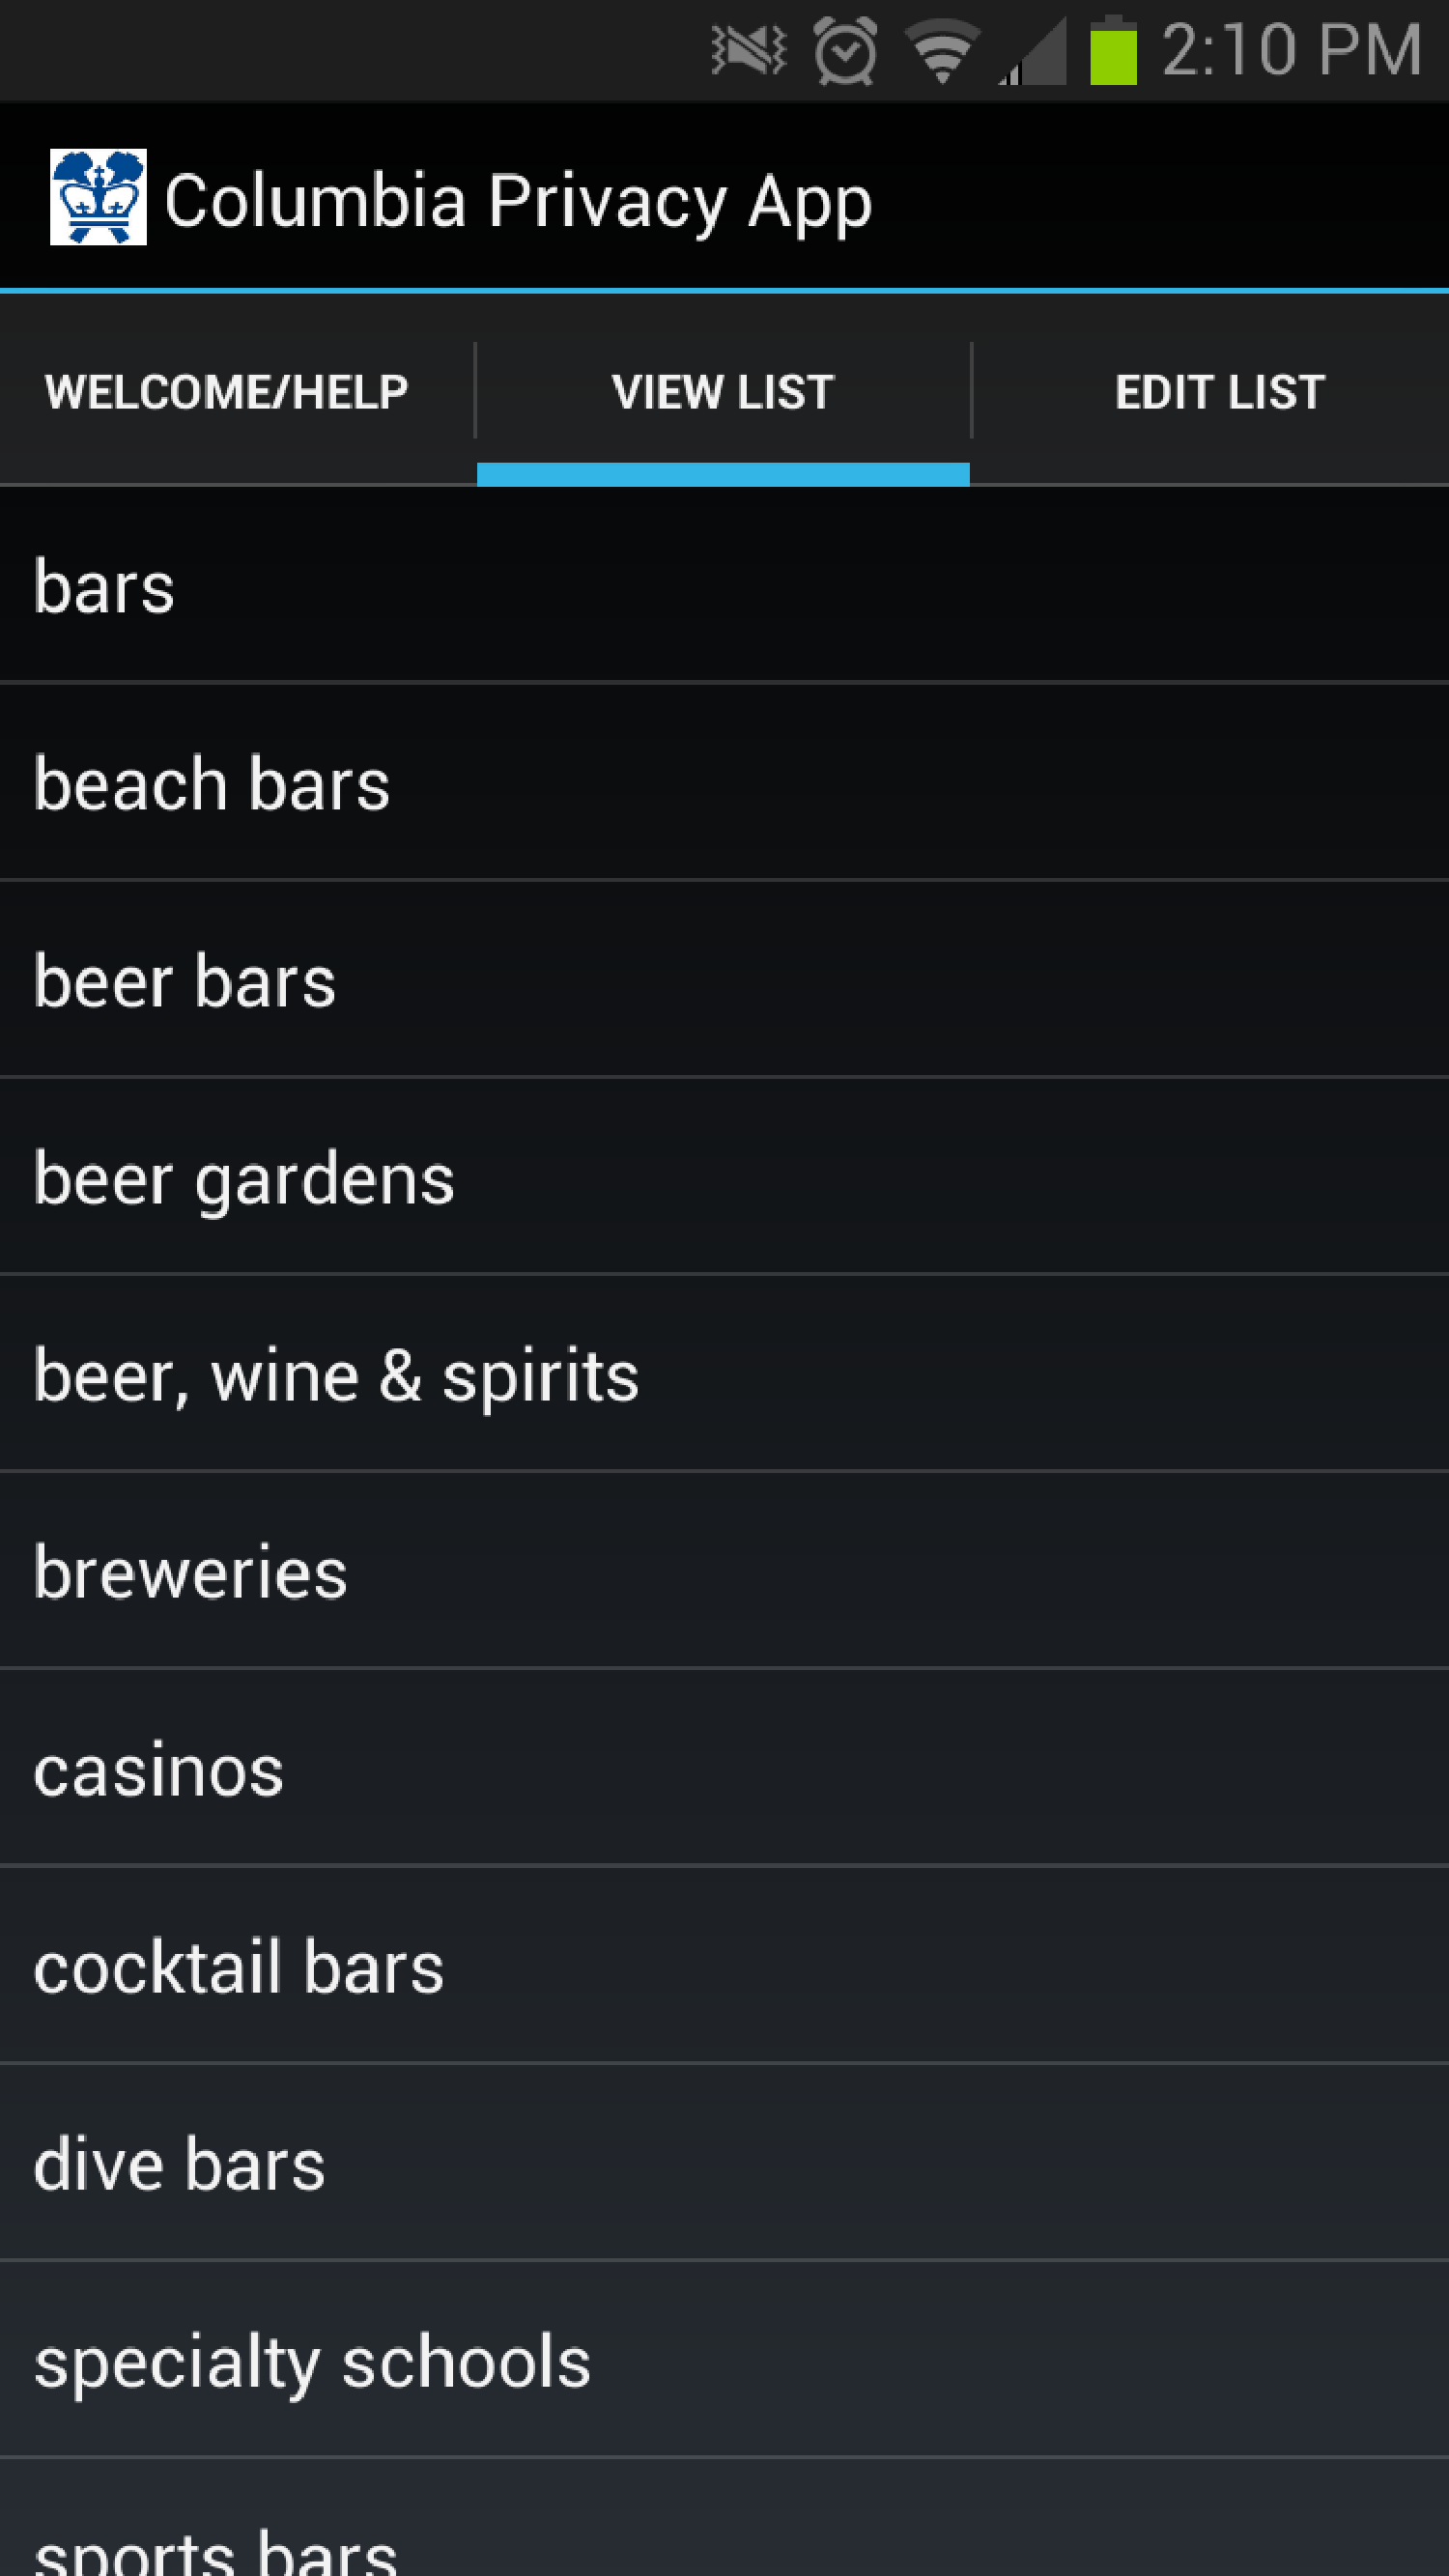
\includegraphics[width=0.75\linewidth]{./fig/screenshot_blacklist.pdf}
%   \caption{Blacklist}\label{fig:awesome_image1}
% \endminipage\hfill
\minipage{0.2\textwidth}
	\centering
  \includegraphics[width=0.75\linewidth]{fig/keyword/screenshot_addlist.pdf}
%  \caption{Adding screen}\label{fig:awesome_image2}
\endminipage\hfill
\minipage{0.2\textwidth}
	\centering
  \includegraphics[width=0.75\linewidth]{fig/keyword/screenshot_map.pdf}
%  \caption{Map}\label{fig:awesome_image3}
\endminipage
\caption{User Interface: (left) managing keywords black list, (right) visualizing locations released.}
\end{figure}
% \end{figure*}

% \begin{figure}[tbp]
% \centering
% \begin{tabular}[1]{cc}
% \hspace{-0.35cm}\includegraphics[width=0.75\linewidth]{./fig/screenshot_addlist.pdf}
% &
% \hspace{-0.35cm}\includegraphics[width=0.75\linewidth]{./fig/screenshot_map.pdf}
% \\
% (a) & (b) \\
% \end{tabular}
% \caption{(a) Blacklist addition screen (b) Map screenshot}
% \label{fig:awesome_image1}
% \end{figure}



% Server-- keywords and storage
% ISSUES: WHAT IF YELP DOESN'T HAVE A BUSINESS? what would a real impkementaiton look like?
% Our \textbf{webserver} had two main functions: reporting a location's keywords and storing a user's public location information.
% To map locations to keywords, we used the Yelp API. \texttt{Yelp.com} is an online ratings and review company.
% Yelp provides a hierarchical list of categories for all locations.~\footnote{Yelp categories: \url{http://bit.ly/12TyTER}}.
% Each time a device uploaded a lat-long to the server, we queried Yelp to find the categories of each location within 50 meters.
% This is a possible area for improvement; in future work, the radius of a query could change depending on an estimate of the device's current accuracy or a user's privacy preferences.
% The categories were then sent to the device.
% In a full implementation, this server should additionally be able to communicate with ad exchanges.

% For the purposes of our small scale user study, we did not create a \textbf{blocking module}. 
% In a full implementation, it would be necessary to block any third-party advertisers who did not participate in the system.
% The connections to ad-networks and aggregators (AdMob, Flurry Analytics etc.) can be blocked by a proxy in the middle and by spoofing the MAC address. 
% All necessary proxies already exist: Privoxy comes with advanced filtering capabilities and handles rewrites of the HTTP headers like the `referrer' header to prevent leakages of any form, and mitmproxy can handle SSL\footnote{\url{www.privoxy.org}, \url{www.mitmproxy.org}}. 
% In addition, as the system works with opt-in users, we can have the users upload their SSH certificates to enable the module in the middle to masquerade as the user. 
% From an application's perspective, no logic is broken. 
% Even for location based services like Foursquare or maps, an unintentional checkin or a search at a private location can be prevented by checking against the blacklist -- an added benefit.  

% Web interface
% The web interface, viewable at \url{keyword.cs.columbia.edu}, displayed all whitelisted locations, both on a map and listed with location keywords and times. In order to protect users' safety, users could contact us at any point if they were concerned about an unintentional location release. Additionally, any time a data point was recorded, we delayed making it public by 24 hours. Users could see their data points in real-time via a password-secured link.

% \begin{figure}[t]
% 	\begin{center}
% 		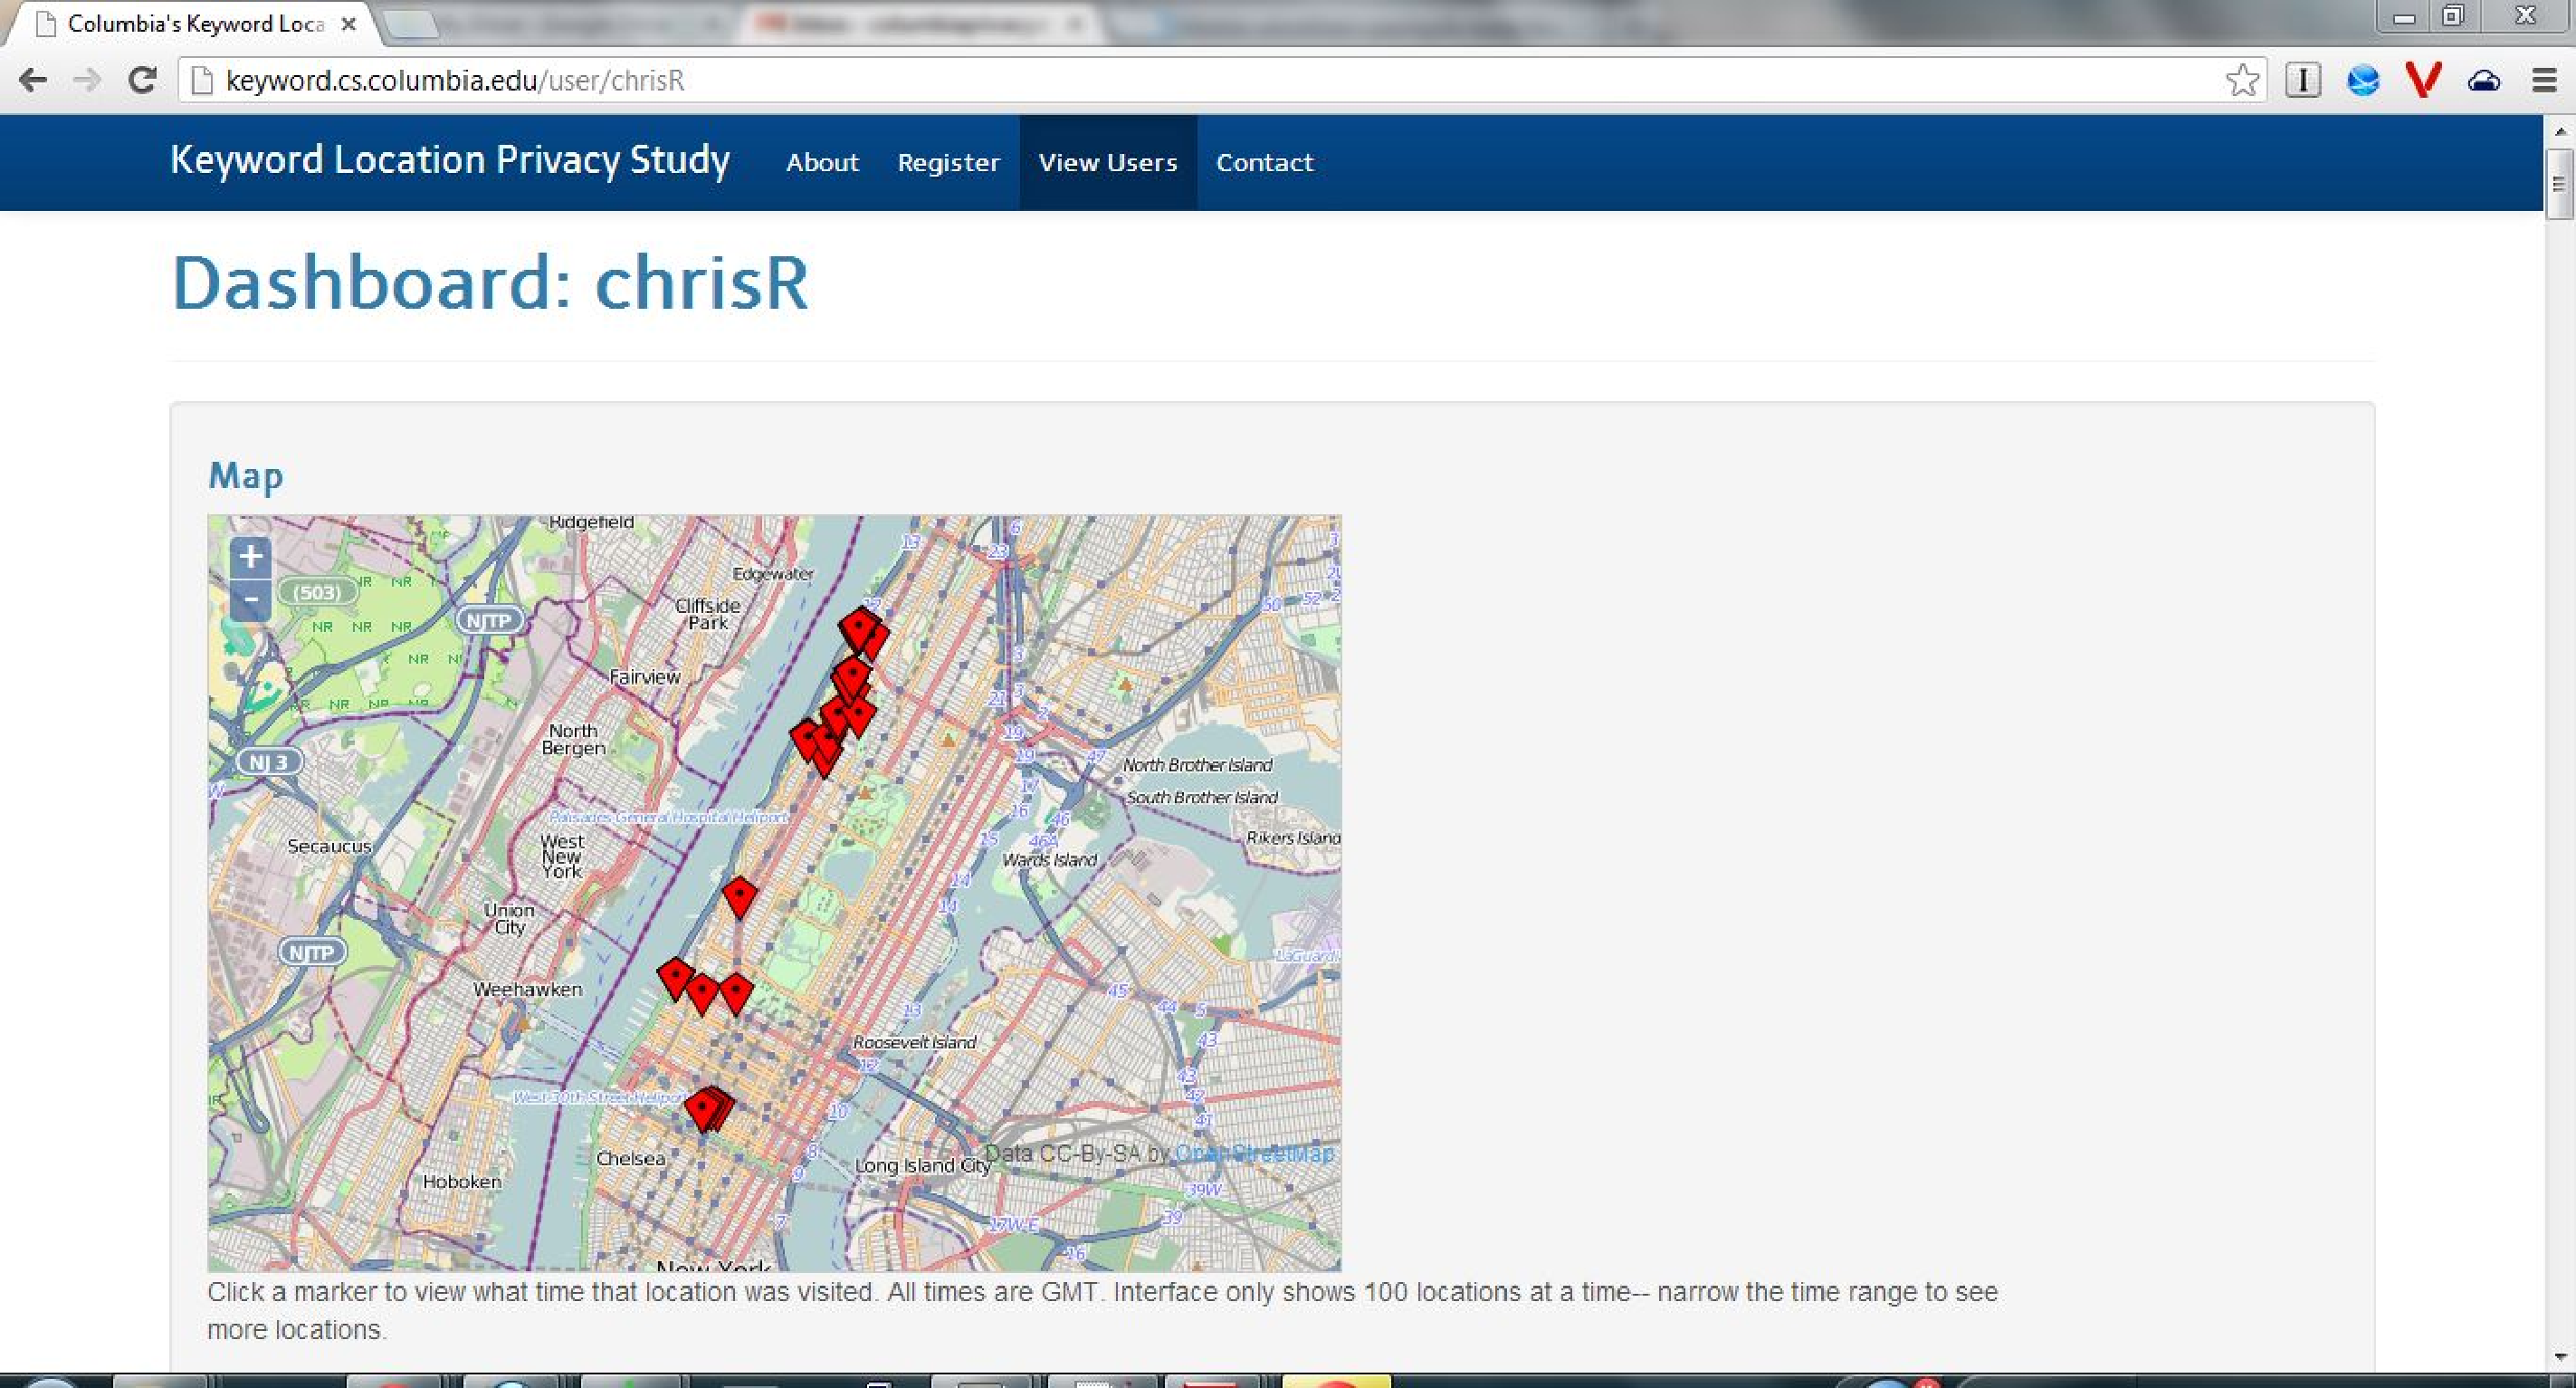
\includegraphics[width=0.9\linewidth]{./fig/web_map.pdf}
% 		% \subfigure[Map view]{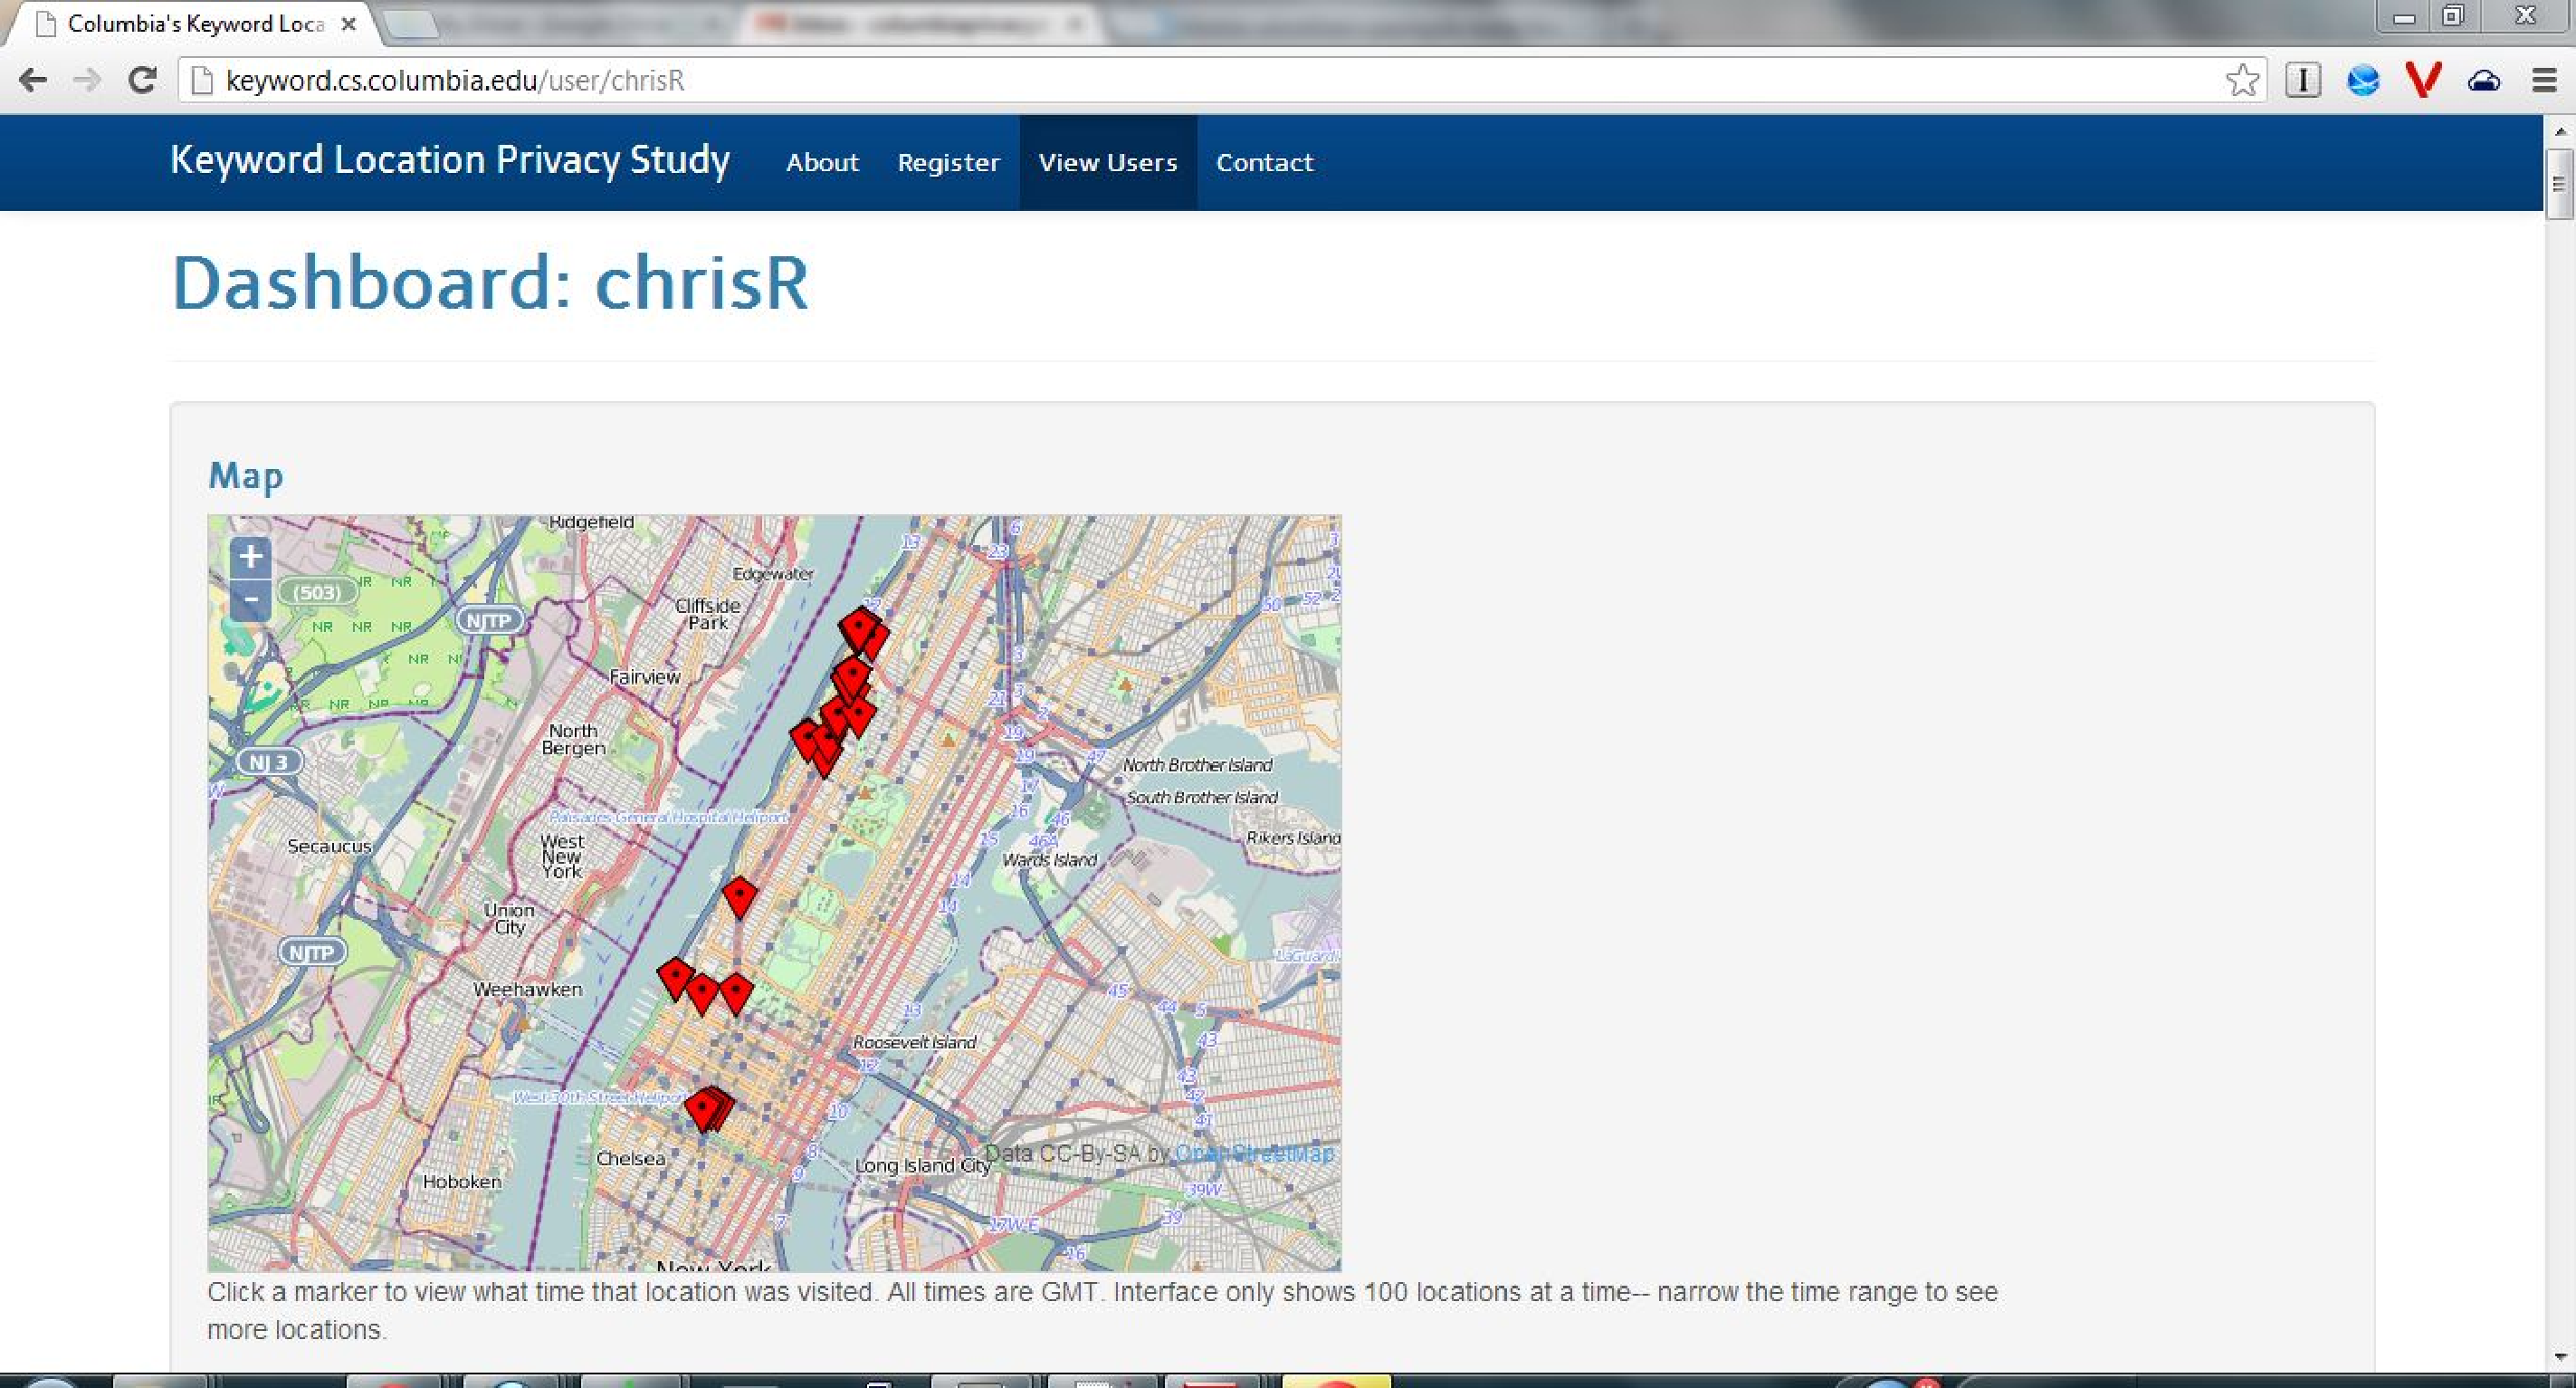
\includegraphics[width=0.9\linewidth]{./fig/web_map.pdf}}
% 		% \subfigure[List view]{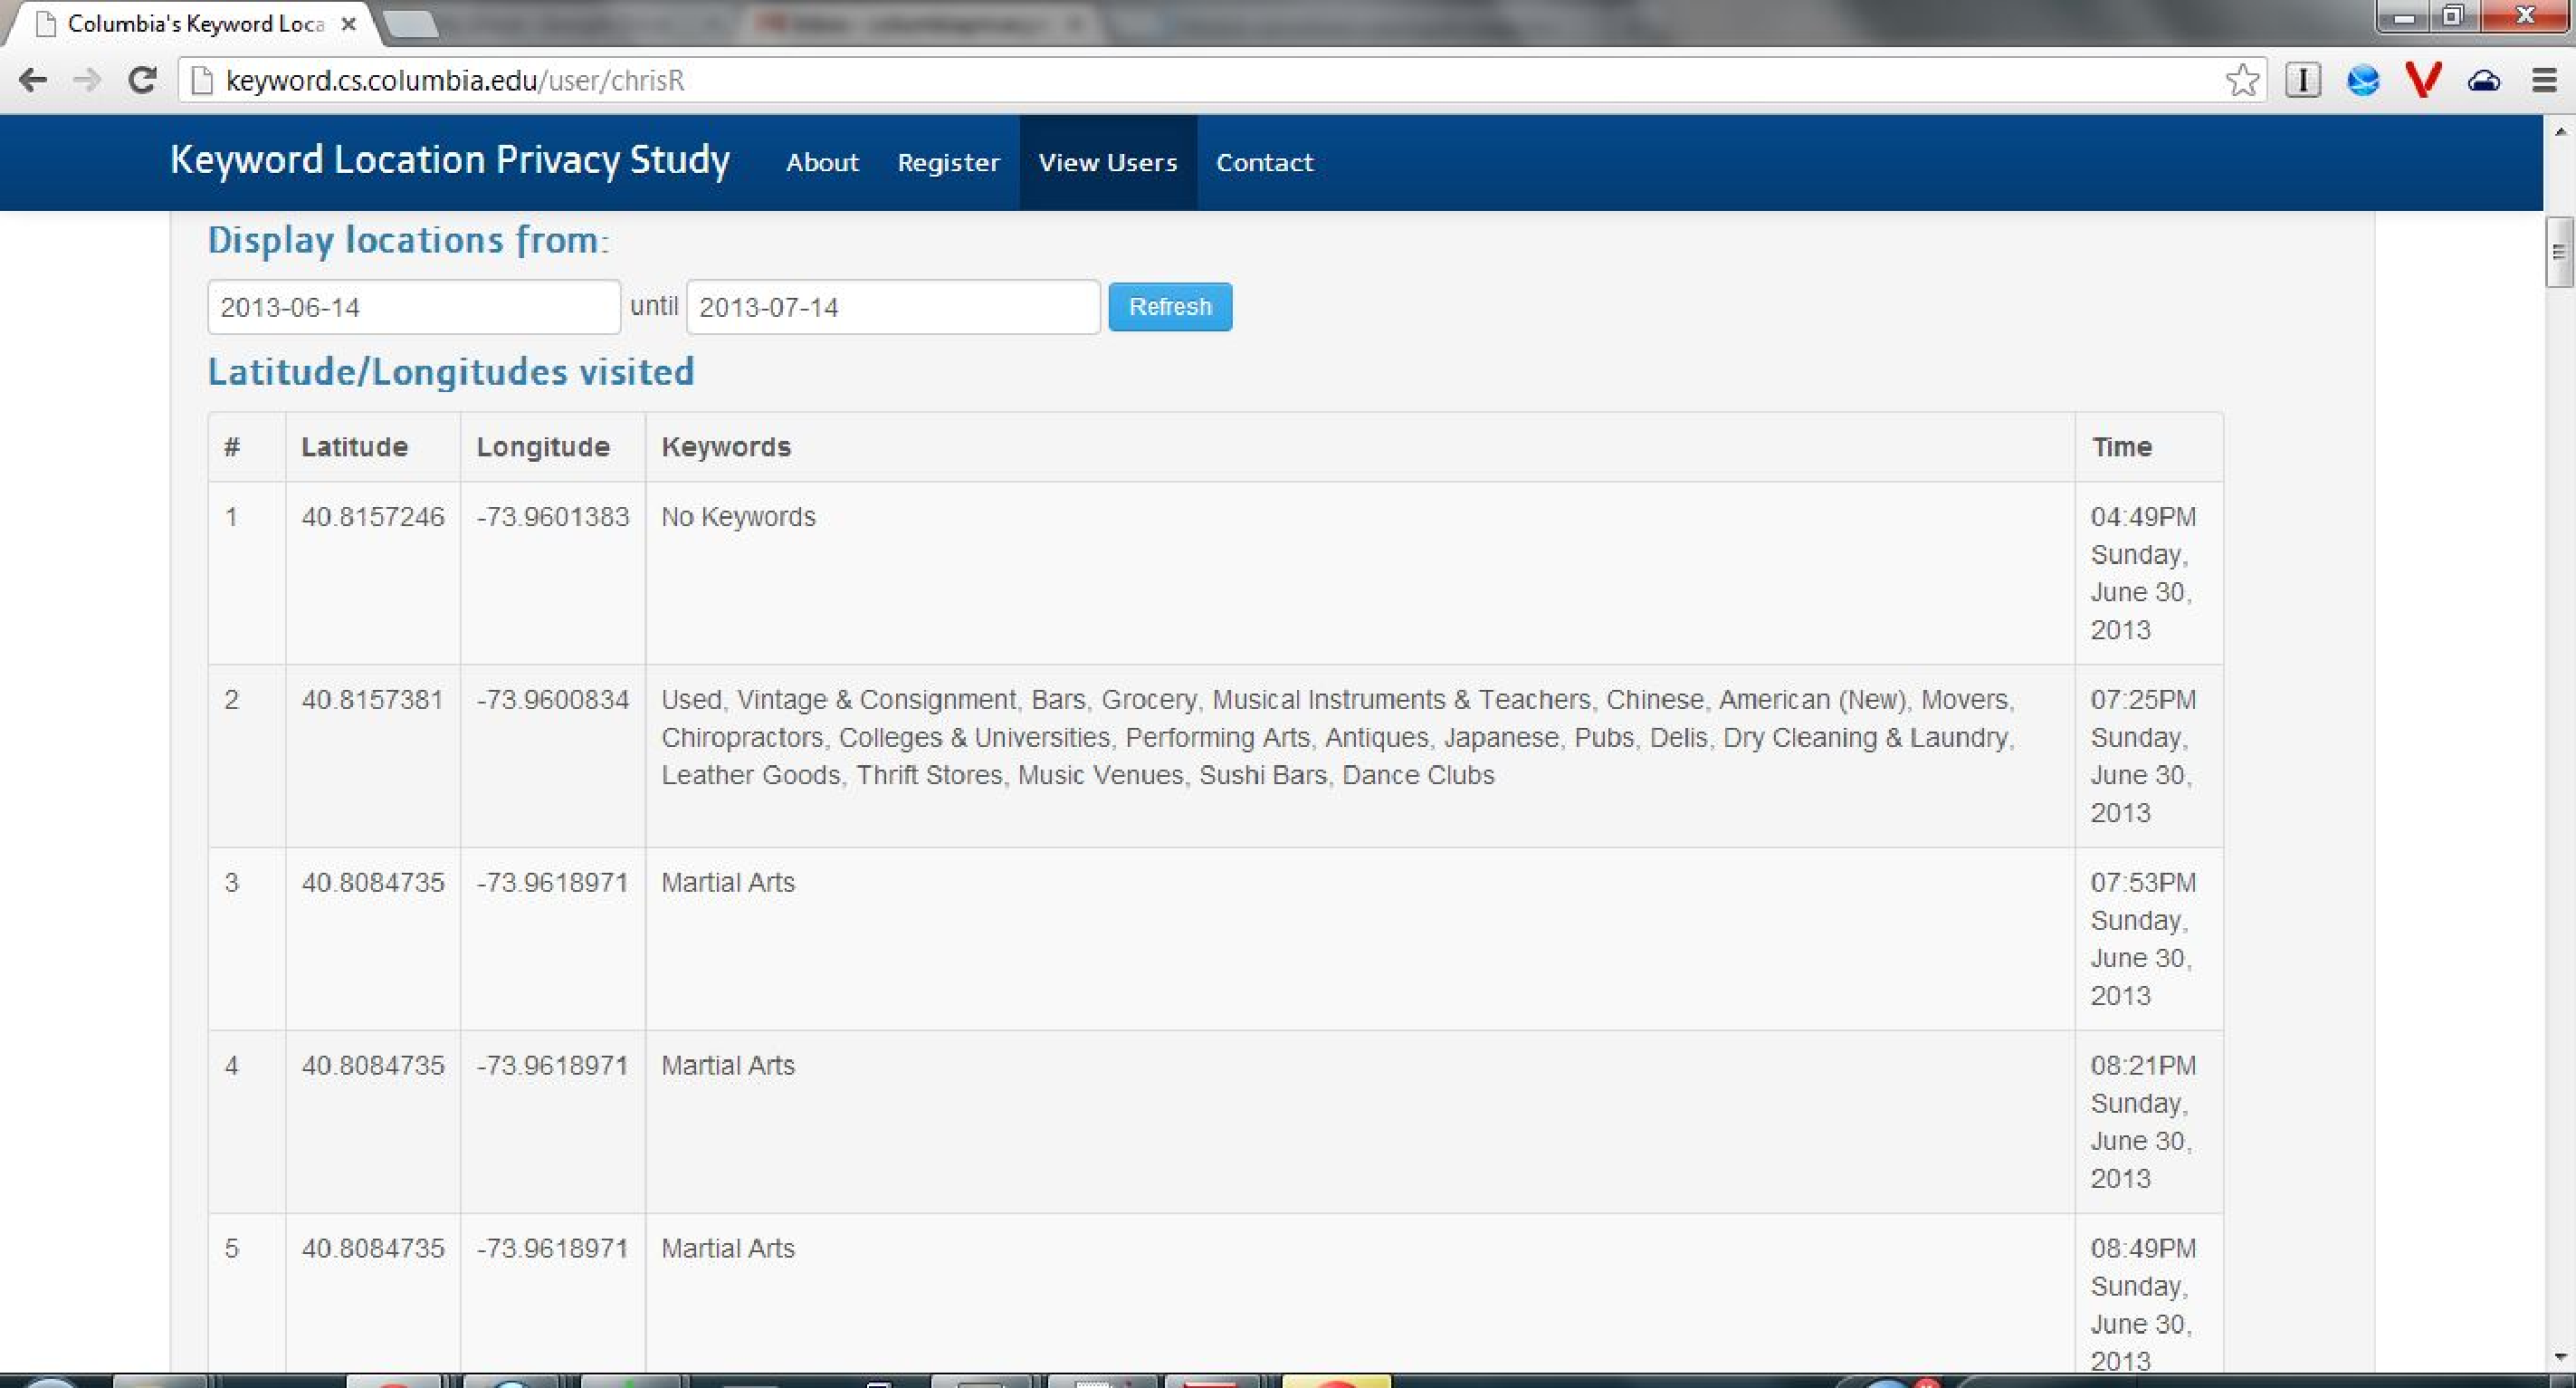
\includegraphics[width=0.9\linewidth]{./fig/web_list.pdf}}
% 	\end{center}
% 	\caption{Screenshot of our web interface (the data shown belong to an author, not a participant).}
% 	% \caption{Screenshot of web interface with one of the author's data. Top: map view. Bottom: list view.}
% 	\label{fig:webInterface}
% \end{figure}

% \subsection{Deployment}

% In a full implementation of our design, advertisers would pay a user whenever they showed an ad to her. 
% As this deployment was meant for exploratory purposes, we did not connect the system to any ad exchanges.
% We instead we simulated the incentives and costs a user might experience while using our system. 
% All participants received a small monetary sum for participating and were entered into a lottery.
% Each user was instructed that releasing more `valuable' information would give them a higher chance of the lottery.
% We did not disclose the exact method of valuing information, mimicking the opaque way in which information would be priced in a real implementation of the system. The intention was that this would incentivize users to release more information.
% % The incentive for a user to release information in our system is money. All participants received \$10 for participating. Additionally, we held a lottery among our users in which the winner would receive \$100. We instructed users that those whose information was more `valuable' would receive more `tickets' in the lottery, and would thus have a better chance of winning. We did not disclose the exact method of valuing information, mimicing the opaque way in which information would be priced in a real implemetation of the system. The intention was that this would incentivize users to release more information.
% To simulate the costs of disclosing information, we publicly displayed a user's non-blacklisted locations on a web interface.
% In a real system, a user would risk that her information is used improperly or released to those who might use it in a damaging way.
% We believed that publicly displaying a user's information accurately simulated this risk. 
% To increase the publicity of their information, we instructed users to post the link on a social media site, such as Facebook or Twitter, and email us a screenshot.

% We deployed our implementation with six users for two weeks. 
% Users were geographically diverse, located in multiple cities throughout the United States.
% % The users were geographically diverse within the USA, including cities on both coasts and the Midwest. 
% % The users were geographically diverse within the USA, including cities on both coasts and the Midwest. 
% Study participants were recruited through advertising on social networks and were primarily adults in their mid-twenties.

% instructions
\subsection{Deployment and Observations}
We deployed our implementation with six users for two weeks. 
Users were geographically diverse, located in multiple cities throughout the United States.
Study participants were recruited through advertising on social networks and were primarily adults in their mid-twenties.

After the study, we asked users to complete a survey. Our study was too small to make general conclusions, 
but we present results here to inform future work. 
% Users easily understood the keyword system and found the interface easy to use. 
Users easily understood both the keyword system and the interface. 
Users were divided on how well they felt the system secured their privacy, with some 
users concerned that our mapping of keywords to locations was not precise enough. Our users expressed a range of 
privacy sensitivities. Some did not use the blacklist and others used the blacklist to hide sites they associated with social stigma or that they thought would send negative signals to employers, insurers or the police.

% We next examined the (non-private) data of our users.
% There was a wide range in the number of locations released by each participant, easily explained by some using the blacklist more than others.
% After running the data through our valuation models, we also saw a wide range in the value across each user's data. 
% As in~\ref{subsec:eval}, we again analyzed the effect of blacklisting on ad revenue by valuing each user's data after removing potentially sensitive information.
% Note that in this case, the user may have already removed some sensitive locations.
% We found that the revenue loss was heterogenous across users: the categories with the largest losses, and the magnitudes of those losses, differed by user.
% When summed, the losses by category appeared to become smoother. This could suggest that a geographically diverse set of individuals will still maintain a good ad revenue despite privacy sensitivities. However, our sample size is to small to make such claims and we leave this question for future work.
 % Contains system description
% % \newpage
\section{Mitigating Attacks}
\label{sec:security}
Having introduced the design of the system, we now turn our focus to one of our key goals: protecting the privacy and value of system participants.
% In this section, we discuss potential attacks that can be made against our solution. 
% Attacks may come from multiple directions-- advertisers trying to gain access to users without paying, malicious attackers trying to undermine the privacy of users, or users trying to unfairly obtain money from advertisers.
% We first note that because our solution requires third party entities to pay in order to access the user, any entity who obtains location
% information must pay in order to monetize that information. Having said that, there can be inference
% based attacks, where blacklisted locations of users can be learned by comparing against other users' information
% or ad-networks can learn more about a user, given that mobility patterns are periodic. We deal with such attacks next.

\subsection{Attacks on the Value of User Data}
% There are a variety of ways ad-networks may try to take advantage of information from the system without properly compensating the user. 
% Our system prevents that such adversary economically benefits from doing so.
% Our system prevents an adversary economically benefiting by doing so.
Our system prevents an adversary from economically benefiting by using information about a user without properly compensating her.

Ad-networks may try to build up interest profiles of users over time in order to better target ads later \emph{without} compensating the user. Even if a user's anonymous ID is changed regularly, human mobility patterns are periodic and somewhat predictable, making it easy to link a current anonymous ID to an older one\footnote{Note this profiling works on \emph{non}-blacklisted locations only.}. Our system does not prevent such profiling, and it even makes it easier as the market announces which data is for sale. However, we ensure that this strategy has no economic benefit, for the following reason: all traffic flows go through a proxy, and an ad network who does not pay will receive the identity and location of a user, but a random temporary ID. Then the ad-network, although it has a rich profile of user $u$, is not able to recognize $u$ as the recipient of an ad. For the same reason, ad-networks do not gain by colluding or reselling the information. Unless a payment is made, the identity and location of $u$ is unknown, and the profile alone does not aid targeting. % suffice to target.

% In any case, an ad-network can only obtain location data if that location does \emph{not} appear on a user's blacklist.
% Thus, any data used to build an interest profile will be data the user is comfortable releasing.
% Because a user's anonymous ID is changed regularly, it takes extra effort on the part of the advertiser to 
% MORE?

A related issue is trajectory-based profiling. If an ad-network learns the habits of a particular user over time, the ad-network can show ads based on where a user \emph{is likely to be} rather than paying for an exact location. Again, ad-networks must always pay to be able to access a user's identity. 
 % only knows that a user visits a location if the user has not blacklisted it.
Care must be taken, however, to make sure that a user does not unwittingly display information about a visited blacklisted location based on her trajectory: \eg~ location B is sensitive and locations A and C are not, and the only way to get to C from A is via B). If Alice checks in at point A and then at point C, ad-networks may infer that she visited B. Such attacks are not likely, and can be dealt with by ensuring that after visiting a blacklisted location a minimum amount of time has passed before disclosing a location. 

One concern is if an app works to circumvent the proxies and leak information about either the location or the identity of the user. 
% Against location leakage, one solution is to not reveal the location to the application if that is doable, and if the OS properly implements a user's privacy preferences. 
Against location leakage, one solution is to substitute a fake location to the app if it does not disrupt service~\cite{Hornyack:2011wq}.
An adversarial app could monitor the location market and try to associate an anonymous user profile with a particular device. Combined with a profiling attack, it can then send targeted advertisements without compensation by recognizing this device from now on. This is a costly attack and can be prevented if OSes separate their advertising services from applications~\cite{Leontiadis:2012} or if the users does not need a permanent ID for this application. Note also that, since UIDs are changed periodically, the profile cannot be updated without paying and hence loses some value over time.
% a user over time, and try to associate a user's anonymous data with a certain device, thus gaining the 

\subsection{Attacks on User Privacy}
\label{sec:inference}

We study the robustness of our solution against a form of attack based on \emph{inference}.
We consider a malicious adversary whose goal is to predict the visits to blacklisted locations of 
a specific user with some accuracy.
This may seem a priori impossible since whenever a user visits a blacklisted location, no information about this visit 
is sent or shared anywhere. 

However, because mobility patterns tend to be periodic and similar people may have similar mobility patterns, an adversary 
may be able to discover something about a specific user's blacklist by comparing their publicly available location information 
with the full (including blacklisted) location information of `compromised users'.
This auxiliary location information could be obtained via hacking or a malicious or buggy application.
% However, one could argue that even if an adversary cannot start from information exchanged in transactional location privacy to make this inference, this adversary might be able in some cases to first gather some partial auxiliary information about some nodes and to \emph{augment} this information using our scheme. 
Inspired by de-anonymization techniques based on auxiliary information~\cite{Narayanan:2008iu}, we now pose the following question:~``Can an adversary with the full knowledge of the location information of a significant 
fraction of users predict the blacklisted locations of other users with high accuracy?'' 
We test this on a large dataset of Foursquare checkins.
Intuitively, the sparsity of locations and checkins in this dataset allows for strong attacks of this kind.

\newcommand{\simil}{\textrm{Sim}}
\newcommand{\spann}{\textrm{span}}
As in the de-anonymization technique, we consider a similarity score $\simil(u,v)$ between two users based on common visits. Let $L_u$ denotes the places that are visited at least $1$ time by $u$. We define similarity as:
\[
\simil(u,v) = \sum_{l\in\setL} \frac{1}{\spann(l)} \mathbb{I}_{l\in L_u\cap L_v} \vf
\textrm{for}\; 
\spann(l) = \sum_{u\in\setU} \mathbb{I}_{\{l\in L_u\}}\ff
\]
Note that by doing so we weight more the co-occurrence of a rare location as a sign of similarity between two nodes.

The attack then proceeds as follows. For a given keyword $k$, the attacker looks at all accounts that visited a location tagged with $k$. For simplicity we will say that such a user visits keyword $k$. These are the probes used to find similar users who are more likely to behave like them. For a given user $u$, the adversary first locates the $n=10$ closest users that are compromised in terms of similarity $v_1,\cdots,v_{n}$. 
The attacker then computes the following weighted sum:
\[
P(u) = 
\frac{1}{\sum_{i=1}^{n} \simil(u,v_i)} 
\sum_{i=1}^{n} \simil(u,v_i) \mathbb{I}_{\{v \midwor{\footnotesize visits keyword}k\}}.
\]
It then predicts that $u$ visits locations associated with keyword $k$ if and only if $P(u)\geq \theta$ where $\theta\in[0;1]$ is a parameter that allows a trade off between accuracy and aggressiveness of the reconstruction technique.

We empirically study the effectiveness of this attack using 1.3 million checkins at 460,663 locations from 40,578 Foursquare users, obtained through crawling publicly available tweets of checkins between March and August 2011. Each Foursquare location is marked with a category, which we assigned to be that location's keyword. In this attack, we consider a severe case where the adversary has compromised 20\% of all accounts. We vary the value of $\theta$ from 0 to 1 and plot the precision-recall of this attack for various keywords in Fig.~\ref{fig:inference}.
\begin{figure}[tbp]
\centering
\begin{tabular}[1]{cc}
\hspace{-0.35cm}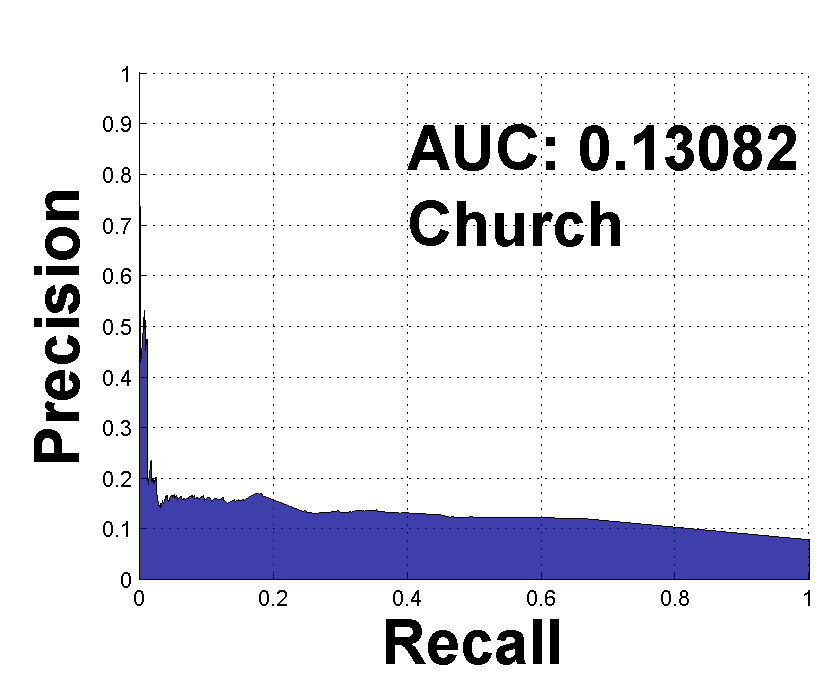
\includegraphics[width=1.5in]{fig/keyword/inf_church_pr.eps}
&
\hspace{-0.35cm}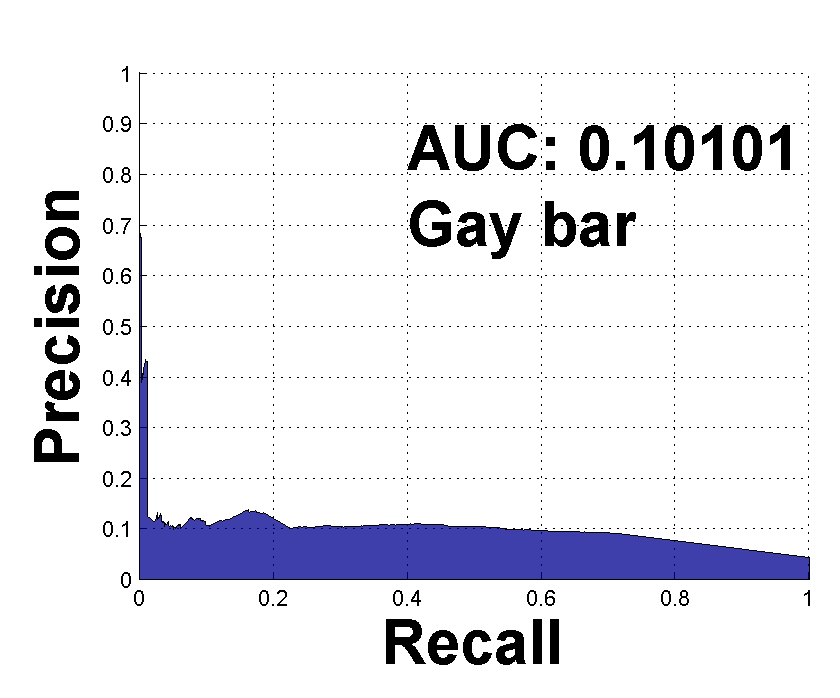
\includegraphics[width=1.5in]{fig/keyword/inf_gaybar_pr.eps}
\\
(a) & (b) \\

\hspace{-0.35cm}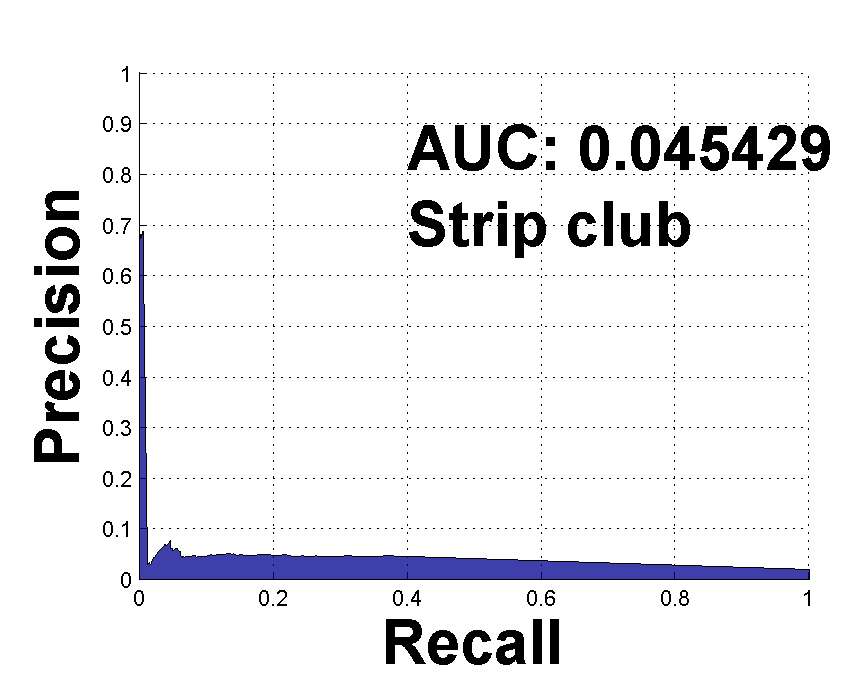
\includegraphics[width=1.5in]{fig/keyword/inf_stripclub_pr.eps}
&
\hspace{-0.35cm}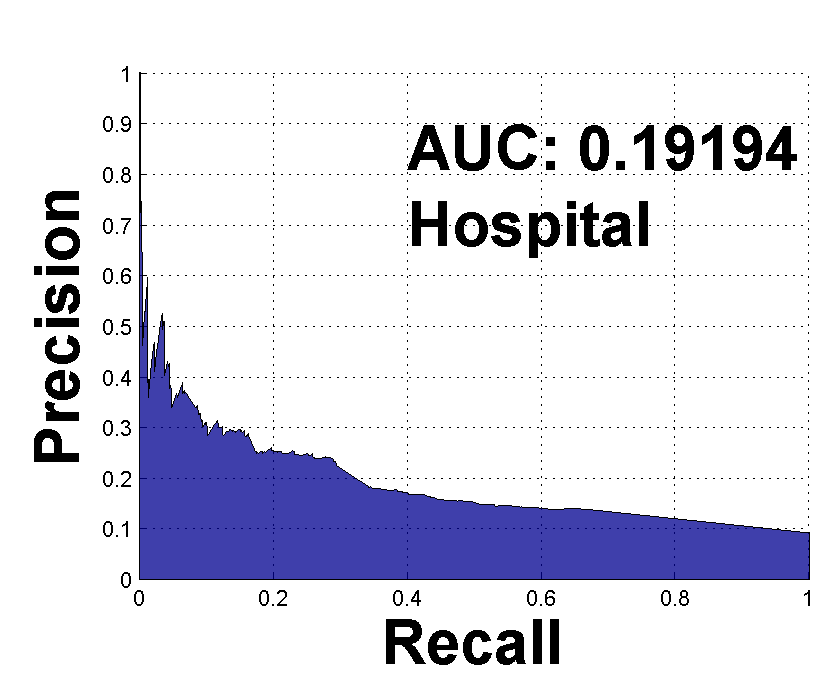
\includegraphics[width=1.5in]{fig/keyword/inf_hospital_pr.eps}
\\
(c) & (d) \\
\end{tabular}
\caption{Precision-Recall curves for four sensitive keywords: (a) Church (b) Gay Bar (c) Strip Club (d) Hospital}
\label{fig:inference}
\end{figure}
As one can see, this attack is rarely effective, even in such extreme case where many user accounts have been compromised. The area under the curve is almost always very small. 
This turns out to be true even for locations that are sparse, as it is much more difficult to guess right when only a handful of users are visiting a rare location. 

This points to an interesting difference between inference in our scheme and de-anonymization attacks. While de-ano\-ny\-mi\-za\-tion attacks always benefit from sparsity since the data are present in a sanitized form, in our context, the attack does not always benefit from sparsity. This is because a minimum critical mass of typical behavior is needed in order to run inference. This shows that a proper choice of blacklist could potentially protect many locations, even as several accounts are compromised in the system. 

% Not sure where Bala wanted me to put this...

% More work remains to be done in this area. 
% One promising direction of study would be the effect of translating locations to keywords on k-anonymity in large traces.
% Another topic to be considered is trade-offs between time granularity and privacy.

\subsection{Attacks on Advertiser Revenue}
We now consider if advertisers can unfairly lose money to unscrupulous users of the system.
Because users are paid when they are accessed by advertisers, they have an incentive to view or click on many ads, even when they are not interested in the displayed products, to artificially boost their profile's value to derive more money from each click.
We label these activities ``user fraud." %different name??

% It is important to note that digital user fraud is really a special case of invalid traffic in online advertising.
User fraud is a special case of invalid traffic in online advertising.
According to Google's Ad Traffic Quality Resource Center, ``invalid traffic includes both clicks and impressions ... [that are] not the result of genuine user interest. This covers intentionally fraudulent traffic as well as accidental clicks and other mechanically generated traffic."\footnote{\url{www.google.com/ads/adtrafficquality/index.html}}
% This definition applies equally well to any clicks or impressions a user creates in order to game the system.
A request for an ad within our system is just like a request for an ad in the current ad ecosystem, but with some privacy-protecting filtering and potential additional location information.
Thus, previous techniques used to identify invalid traffic can be used to identify user fraud.
% Recently, there has been a variety of research on this subject.
There is a lot of recent research on this topic.
Dave et al propose methods to fingerprint click spam~\cite{clickspam}.
Haddadi uses ``bluff ads", ads designed to not appeal to humans and thus only be clicked by bots, to defeat click fraud~\cite{bluffad}.
Information on the structure of Google's click fraud detection system is available ~\cite{googleClick1}. %, ~\cite{laneGiftReport}.
Beyond academia, multiple startups exist that estimate the rates of click fraud,
such as Adometry, Visual IQ, and ClearSaleing~(%\footnote{
\url{www.adometry.com}, \url{www.visualiq.com}, \url{www.clearsaleing.com}
%}
).
% We first note that such a problem is only as difficult as that of standard click fraud on the web.
% The amount of money to show one impression of an ad on the internet is exceedingly low, meaning the amount of money a user can expect to get from viewing an impression in our system will also be low.
% Thus, we only need to worry about 

Additionally, it is easier to detect user fraud than traditional invalid traffic because location information is more constrained than web-browsing.
Users are physically constrained in how far they can travel in a certain period of time
and typically display periodic mobility patterns, returning to their homes at night and spending week days at work locations.
A more extreme use of physical constraints would be to use location tags; fingerprints extracted from ambient signals at a specific location at a specific time~\cite{NarayananTLHB11}.
These constraints can be used to filter out automated attacks on a system. 
For example, if a user appears to be traveling faster than is physically possible, we can remove them from the system or verify their accounts with a Captcha or phone call.
Because of these physical constraints, and because click fraud prevention techniques can easily be applied to our system, we believe that our system is no more vulnerable to gaming than current online advertising. 
% Although click fraud is considered an open problem by the research community, 
The ongoing viability of online advertising shows that our solution should likewise not be derailed by invalid traffic.

% Beyond digitally generated location fraud, 
Beyond automated attacks, users might ``physically" attack the system by simply going to a high value location in order to appear more valuable to an advertiser than they actually are.
Again, techniques to combat click fraud can be employed here.
Click fraud techniques must deal with situations in which users actually click links to unfairly gain money, a nice analogy to this form of attack.
Beyond this, traveling to a location takes significant time and effort and will likely be too costly to be a viable way of making money.

% Traveling to a location takes significant time and effort. Such time and effort has an opportunity cost. 
% In order to make such an attack worthwhile, the user would have to have a very valuable profile. We don't anticipate profiles having such a high value unless the user has made multiple purchases in the past, in which case the advertiser would be compensated appropriately.
% Finally, the market should help deal with these attacks. We believe that valuable profiles will be distinguishable from worthless ones. The market should then be able to appropriately price them. To aide in this distinction, some reputation scheme could be added on top of the user's profile. For example, a user could receive a rating based on how often they respond to advertising.

% Gaming of the system is certainly an issue and an area for future study. 
% However, we believe that such concerns are no more difficult than the current click fraud situation facing online advertising.
% Given that online advertising is a thriving field in spite of these concerns, we feel that gaming does not pose a disastrous risk to our system.

% \section{Related Work}
\label{sec:relwork}

%We have presented an economic solution to location privacy that we refer to as
%transactional location privacy. Our solution has a economic component that
%associates a value to each location disclosure and a systems component that 
%helps maintain privacy. 

%Lot of work has been done on the economics of information disclosure~\cite{Ghosh:2011jy, Cvrcek:2006vv, Danezis:2005wq}.
%Ghosh et al. discuss and analyze economic value of information as treated by differential privacy~\cite{Ghosh:2011jy}. 
%Our work is different in that we focus on location information and we stress releasing non-obfuscated, pure information, instead of adding noise to a release as differential privacy dictates. 
%We believe releasing raw data is crucial for any solution to be supported by web service providers. 
%Carrascal et al~\cite{Carrascal} utilized experience sampling to study how users value their personal information online.
%Danezis et al studied specifically the worth of location information from
%the perspective of users~\cite{Cvrcek:2006vv, Danezis:2005wq}.
%Our work seeks to create a market that determines a price for user data based on what companies are willing to pay and what consumers are willing to receive.
%% Our work is complementary as we develop a model to quantify how much location is worth from the perspective of ad-networks and aggregators.

Our work is part of a growing body of work that deals with privacy solutions that aim to reconcile the privacy concerns of users with the economic needs of `free' online web services and mobile applications~\cite{Guha:2011wj, guha:koi, Riederer:2011ta, Toubiana:2010tm}. 
Privad~\cite{Guha:2011wj} and Adnostic~\cite{Toubiana:2010tm} are browser based systems that enable behavioral targeting while ensuring users' PII is not leaked to ad-networks performing the targeting. 
Our focus in this paper is different -- we are concerned with location information on mobile devices. 
Koi~\cite{guha:koi} is a system developed to address location privacy by way of location matching -- applications and service providers pre-declare which locations they would be interested in and the device releases this information at those specified locations. 
Our solution is different, in that we have an economic component where application developers need to pay
to access the user at the specified location. 
In addition, neither the device nor applications have to be modified to use our solution. 
% We believe incentives of economic gains are much stronger to increase adoption of a privacy solution. 
Our work is closely related to transaction privacy~\cite{Riederer:2011ta}.
The difference is that we focus on location information for mobile devices and develop a keyword-based disclosure scheme.
% an economic model of location information to drive our market. 

% With less econ, this is deemphasized a bit...
% Bacelli et al~\cite{infocom:fb} authors propose models to quantify the economic value of various locations, with the specific example of proximity advertising in mind.
% With regards to the economic valuation of location information, the closest work to ours is the work by Bacelli et al~\cite{infocom:fb} where the authors propose models to
% This is similar to our proposal, in that we too focus on proximity advertising and are interested in real-time location information. 
% The main difference is that our approach is more empirically driven and much simpler with fewer assumptions. We rely on keywords associated with locations (derived from real data) and make no assumptions on how various businesses are distributed in a geographical region.  
% We focus more on intent, captured by frequency of visits to a location, to approximate interest in a location and the propensity to conduct a commercial transaction at that location.
% Bacelli et al rely on a set of interests of a user that are known to the model.

% \section{Conclusion}
\label{sec:conclusion}

The collection and monetization of location information has become a large concern. % for privacy advocates and regulatory bodies. 
The main contribution of this paper is the design and analysis of a solution for location privacy using economics.
Our solution is simple -- opt-in users decide which locations to reveal and only these locations are sold on an information market. 
Buyers pay to gain access to users at specified locations.
Locations are specified in keywords, a notion intuitive to both end users and advertisers.
Our solution relies on a privacy protection component that ensures that the location information the user chooses not to release will not be leaked, and also minimizes the linkage of the user's identity with the released information. 
Future research  directions on keyword-based disclosure may include reducing the role of the trusted third party, larger implementations, and a stronger economic analysis of the solution.
A few locations, at a cell level, have been shown to provide poor anonymity~\cite{de2013unique}.
An interesting open question is if keywords provide better k-anonymity.

% We find that in terms of the value of location information, very few locations (5\%) account for majority of the value.
% We find that potentially sensitive locations (as defined by sociological research) appear to be well distributed across locations sorted by popularity and profitability.
% Likewise, we find that the potential revenue of these sensitive locations is small compared to the total value generated from all locations. 
% This suggests a sweet-spot between location privacy and monetizing location information.
% We construct and deploy a small scale version of the system with real users, showing that our solution is indeed feasible.
% We observe their behaviors and lay the groundwork for future study.

